\documentclass{sig-alternate}

\usepackage{graphicx}
\usepackage{amsmath}
\usepackage[caption=false,font=footnotesize]{subfig}

\DeclareMathOperator{\median}{median}
\DeclareMathOperator{\dis}{d}
\DeclareMathOperator{\mad}{MAD}

\title{Strip, Bind, and Search: A Method for Identifying Abnormal Energy Consumption in Buildings}
% Mining Devices Intrinsic-Relationships to Identify Energy Saving Opportunities in Buildings


\author{
Romain Fontugne{\large$^{1,5}$}, Jorge Ortiz{\large$^2$}, Nicolas Tremblay{\large$^3$}, Pierre Borgnat{\large$^3$}
\\
Patrick Flandrin{\large$^3$}, Kensuke Fukuda{\large$^4$}, David Culler{\large$^2$} and Hiroshi Esaki{\large$^1$}
\\~\\
{\large$^1$}The University of Tokyo~~~~~{\large$^2$}University of California, Berkeley\\
{\large$^3$}CNRS, Ecole Normale Sup\'erieure de Lyon~~~{\large$^4$}National Institute of Informatics\\
{\large$^5$}Japanese-French Laboratory for Informatics
}

\begin{document}

\conferenceinfo{IPSN'13,} {April 8--11, 2013, Philadelphia, Pennsylvania, USA.} 
\CopyrightYear{2013} 
\crdata{978-1-4503-1959-1/13/04} 
\clubpenalty=10000 
\widowpenalty = 10000


\maketitle

\begin{abstract}
% % Buildings in the United State consume 41\% of the total energy produced.
% % In order to reduce the electrical footprint of buildings we present a new methodology to monitor building consumption and identify saving opportunities.
% % The proposed method uncovers the relationships between the building's electrical devices and determines the devices normal behavior.
% % Furthermore, by monitoring the devices relationships over time and comparing it to their usual relationships the misbehaving devices are automatically identified.
% % We demonstrate that these misbehaviors correspond to incorrect usages of the devices thus sources of electricity wastes.
% % The main challenge in this approach is to retrieve devices intrinsic-relationships from the sensor raw data.
% % Indeed these relationships are hidden by noise and common trends inherent to all the sensors in the building.
% % We overcome this issue by filtering the raw data using a recent signal processing technique: Empirical Mode Decomposition.
% % The proposed method is evaluated with 18 weeks of data from two buildings located in U.S. and Japan.
% % In spite of the national post-Fukushima measures to reduce the electricity consumption in Japan the proposed method found several saving opportunities in the Japanese dataset.
% % In the other dataset it also detected several electricity wastes that account for up to 2500~kWh.
% 
% A typical medium-to-large building %($\geq 10^{5}$ square-feet) 
% contains thousands of sensors, monitoring the HVAC system, lighting, and
% other operational sub-systems.  With the increased push for operational efficiency,
% operators are relying more on historical data processing to uncover opportunities for savings.  
% However, they are overwhelmed 
% with the deluge of data and seek more efficient ways to identify potential problems.  In this paper we present a new approach,
% called the Strip and Bind Method (SBM), for uncovering potential problems in equipment behavior and in-concert usage.  
% SBM uncovers relationships between devices and constructs a model for their in-concert usage.  It then flags deviations from the model as abnormal.
% 
% Unlike other approaches, SBM requires no a priori 
% knowledge about the building and runs on all sensors data -- treating each stream as a time-varying signal.
% % Since most sensors in the building are driven by the same underlying activity and weather patterns, we first had to remove
% % the dominant trend to obtain the instrinstic behavioral pattern.  Detrending is done using 
% % Empirical Mode Decomposition -- a recent signal processing tool.  We then construct a correlation-based model on the underlying 
% % intrinsic signals. 
% We run SBM on a set of building sensor traces; each containing up to several thousand sensors and over 500 GB of data, collected over
% 18 weeks from two separate buildings in different geographic locations and climates.  We demonstrate that, in many cases, SBM uncovers
% misbehaviors correspond to inefficient device usage that leads to energy waste.  The average waste uncovered is as high as 2500 kWh per 
% device.


A typical medium-to-large building contains thousands of sensors, monitoring the HVAC system, lighting, and other operational sub-systems.
With the increased push for operational efficiency, operators are relying more on historical data processing to uncover opportunities for energy-savings.
However, they are overwhelmed with the deluge of data and seek more efficient ways to identify potential problems.
In this paper we present a new approach, called the Strip and Bind Method (SBM), for uncovering relationships between devices and model their in-concert usage.
A longitudinal analysis of building data using SBM permits to determine the normal behavior of the devices and flags anomalous device usages.
Unlike other approaches, SBM requires no a priori knowledge about the building.
We run SBM on a set of building sensor traces; each containing hundred sensors reporting data flows over 18 weeks from two separate buildings with fundamentally different infrastructures.  
We demonstrate that, in many cases, SBM uncovers misbehaviors corresponding to inefficient device usage that leads to energy waste.  
The average waste uncovered is as high as 2500 kWh per device.
\end{abstract}


\section{Introduction}
Buildings are one of the prime targets to reduce energy consumption around the world.
In the United States, the second largest energy consumer in the world, buildings account for 41\% of the country's total energy consumption \cite{aer2011}.
The first measure towards reducing the building's energy consumption is to prevent electricity waste, due to the improper use of the buildings equipment.

Large building infrastructure is usually monitored by numerous sensors.
Some of these sensors enable building administrators to view device power-draw in real time.  This allows administrators
 to determine proper device behavior and system-wide inefficiencies.
%,  and identify devices providing inappropriate services.
% sensors providing a service is weird to think about  -- i like how the next paragraph explains it
Detecting misbehaving devices is crucial, as many are sources of energy waste.  % a light not turning on properly is NOT WASTEFUL, but does affect service quality
However, identifying these saving opportunities is impractical for administrators because large buildings usually contain hundreds of monitored devices
producing thousands of streams and it requires continuous monitoring. % attention as abnormal usages may happen at any time.
%Consequently, the goal of this work is to establish a methodology that reports to building administrators devices abnormal uses.  
As such, the goal of this work is to establish a method that reports abnormal device-usage patterns to the administrator by closely examining 
all of the continuous power streams.

The intuition behind the proposed approach is that each service provided by the building requires a minimum subset of devices.
The devices within a subset are used at the same time when the corresponding service is needed and a savings opportunity is characterized by the partial activation of the devices.
For example, office comfort is attained through sufficient lighting, ventilation, and air conditioning.
These are controlled by the lighting and HVAC system.
%controlled by the lighting system and air conditioner.% the light and air conditioning.
Thus, when the room is occupied both the air conditioner (heater on a cold day) and lights are used together and should be turned off 
when the room is empty.
In principal, if a person leaves the room and turns off \emph{only} the lights then the air conditioner (or heater) is a source of electricity waste.

Following this basic idea we propose an unsupervised methodology to systematically detect electricity waste.
Our proposal consists of two key components:
% \begin{enumerate}
%  \item The strip and bind method (SBM) mines raw sensor data, identifying devices that are used in concert.
%  It uncovers the devices relationships by looking at the correlation of their activities. 
%  Therefore it allows us to differentiate the devices that are used all together (high correlation), devices used independently (no correlation) and the mutually exclusive usages of devices (negative correlation).
%  \item The anomaly detector monitors devices relationships over time and reports misbehaving devices.
%  It learns the devices normal usages using a robust and longitudinal analysis of the building data and detect anomalous usages that stand for electricity wastes.
% \end{enumerate}

\begin{enumerate}
 \item The strip and bind method (SBM) mines the raw sensor data, identifying inter-device usage patterns. % that are typically used in concert to provide a service.
We first \emph{strip} the underlying traces of occupancy-induced trends.  Then we \emph{bind} device traces, whose underlying behavior
is highly correlated, by placing them into a correlated device set.
 %  Then
 % It uncovers the devices relationships by looking at the correlation of their activities. 
 This allows us to differentiate between devices that are used together (high correlation), used independently (no correlation), and used mutually exclusively (negative correlation).
 \item The anomaly detector monitors devices relationships over time and reports deviations from the norm.  % misbehaving devices.
 It learns the normal inter-device usages using a robust, longitudinal analysis of the building data and detect anomalous usage patterns.  Such patterns present an opportunity to reduce electricity waste.
 % that may represent that stand for electricity wastes.
\end{enumerate}

The main challenge we overcame with our approach is uncovering the device relationships from numerous, noisy sensor traces
that all share a similar trend.
%The main difficulty in this approach is to uncover the devices relationship from the numerous and noisy sensor traces. 
Since device energy consumption is mainly driven by building occupancy, all the devices follow the same daily pattern, 
in roughly overlapping time intervals and phases.
%and seem to be used all at once.
Therefore, one of the main contributions of this work is uncovering the intrinsic device relationships by filtering out the dominant
trend.  This is achieved by using Empirical Mode Decomposition \cite{huang:emd1998}.

Another key contribution of this work is in using the SBM method to practically reduce building energy consumption.
Moreover, the proposed method is easy to use and functions in any building, as it does not require prior knowledge of the
 building nor extra sensors.  It is also tuned through a single intuitive parameter.  %which parameter?

We validate the effectiveness of our approach using 10 weeks of data from a modern Japanese building containing 135 sensors and 
8 weeks of data from an older American building containing 70 sensors.
These experiments highlight the effectiveness of SBM to uncover device relationships in a large deployment of 135 sensors.
Furthermore, we inspect the anomaly detector results and show that the reported alarms correspond to significant opportunities to save energy.
The major anomaly reported in the American building accounts for a waste of 2500 kWh over 18 days whereas the building average power consumption is 600 kW per hour.
Without the proposed method identifying these energy wastes would be difficult for building administrators as they are hidden in the building overall consumption.

In the rest of this paper, we detail the mechanisms of SBM and the anomaly detector before evaluating both of them with real data then we discuss different outcomes of the proposed methodology and conclude.


\section{Problem description}
% \subsection{Dominant patterns}
\begin{figure}
\begin{center}
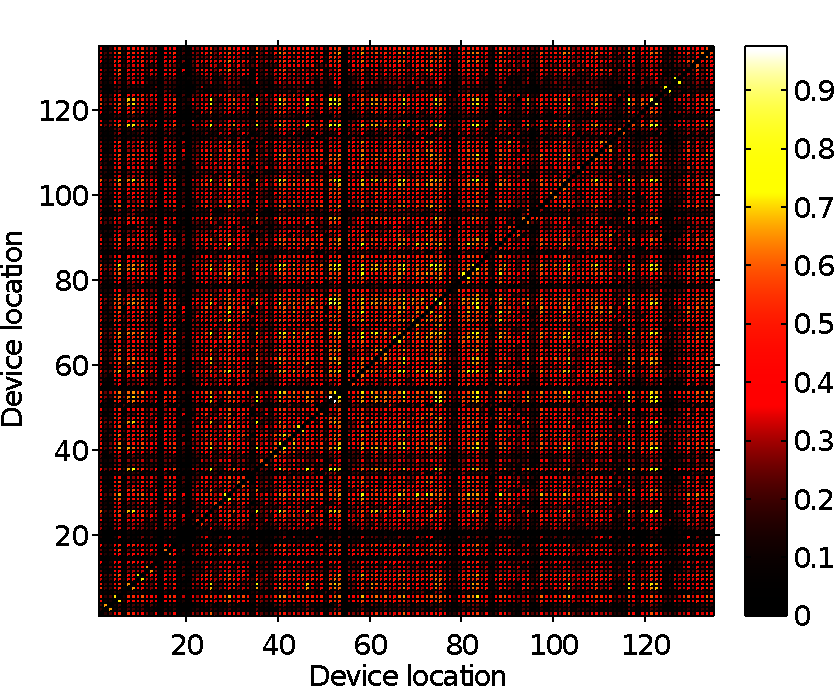
\includegraphics[width=.45\textwidth]{img/heatMap_raw_201106-eps-converted-to.pdf}
\caption{Correlation coefficients of the raw traces from the Engineering Building 2 dataset (Section \ref{data:engbldg2}).
The matrix is ordered such as the devices serving same/adjacent rooms are nearby in the matrix.}
\label{fig:heatmap:raw}
\end{center}
\end{figure}

%The first step of the proposed approach is to uncover from the raw data the devices that are used all together.
The primary objective of SBS is to determine the devices that are used simulataneously.
%The basic tool that allows us to compare device energy consumption is the correlation coefficient.
Initially, we ran correlation analysis across pairs of power-draw signals between distinct devices, summarized by
a correlation coefficient.  However, our results did not yield any useful information when applied to 
the raw data.
%However, during our experiments we found that it provides poor help when it is directly applied to the raw signals.
For example the two raw signals of Figure \ref{fig:diagram1} are from two independent HVAC systems serving different rooms on different floors.
Since each space is independently controlled, we expect their power-draw signals to be uncorrelated (or at least distinguishable 
from other signal pairs).  However, their correlation coefficient ($0.5675$) was not particularly informative.  
% however, their correlation coefficient (i.e. $0.5675$) indicates the opposite.
%Another example, with 135 devices, is depicted in Figure \ref{fig:heatmap:raw}.

% Another example, depicted in Figure \ref{fig:heatmap:raw}, shows a correlation matrix with 135 distinct locations, each containing a number of devices.  
Another example, depicted in Figure \ref{fig:heatmap:raw}, shows a correlation matrix with 135 distinct lighting and HVAC systems serving numerous rooms in a building (Section \ref{data:engbldg2}).
The indices are selected such that their index-difference is indicative of their relative spatial proximity.  
For example, a device in location 1 is closer to a device in location 2 than it is to 
a device in location 135. 
% We do not account for obstructions between them, such as walls.  %?
The color of the cell is the average pairwise correlation coefficient for devices in the row-column index.  The higher the value, the lighter the color.
%the devices serving the same (or adjacent) room are close
%to one another in the matrix.  
Devices serving the same room are along the diagonal.  Because these devices are used simultaneously, we expect
high average correlation scores, lighter shades, along the diagonal figure.
%and because they are used simultaneously by the room users we expect them to feature the highest correlation scores.
However, we observe no such pattern.  %structure is unseen in the Figure.  
Most of the signals are correlated with all the others and we see no discernable structure.
% thus this metric prevents us from finding devices that are used in concert.

\begin{figure}[t!]
\begin{center}
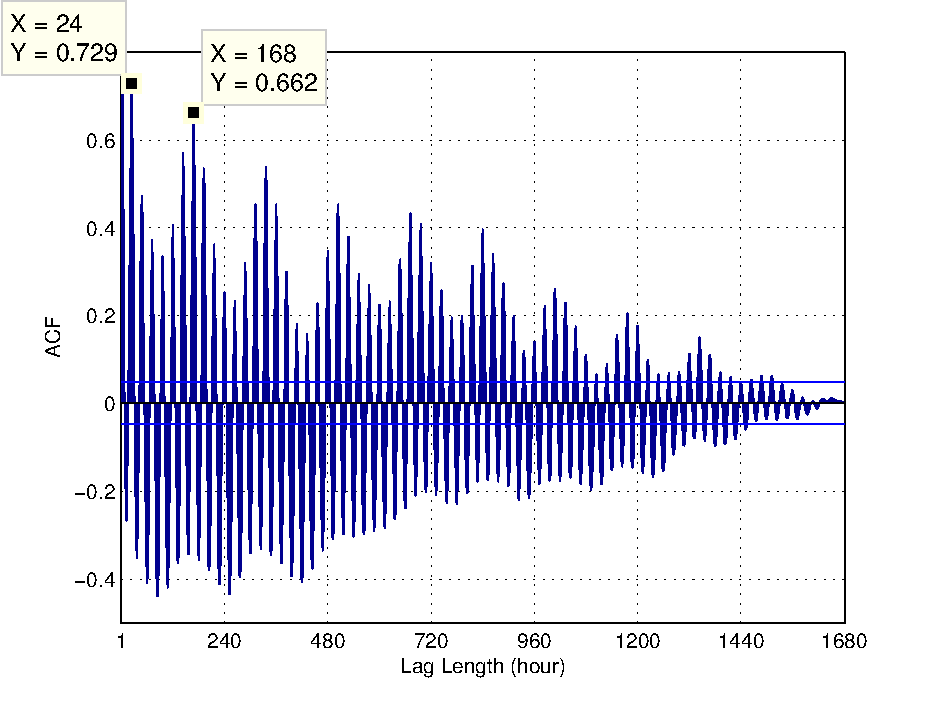
\includegraphics[width=.45\textwidth]{img/acf_101A1_GHP-eps-converted-to.pdf}
\caption{Auto-correlation of a usual signal from the Engineering Building 2 dataset.
The signal features daily and weekly patterns (resp. $x=24$ and $x=168$).}
\label{fig:autocorr}
\end{center}
\end{figure}

Intuitively, the daily occupant usage patterns %office hours, 
drives these results.
Figure \ref{fig:diagram1} demonstrates this more clearly.  It shows two 1-week raw signals traces which feature the same 
diurnal pattern.  
This trend is present in almost every sensor trace, and it hides 
the smaller fluctuations providing more specific patterns driven by local occupant activity.  Upon deeper inspection, we uncovered several
 dominant patterns, common among energy-consuming devices in buildings~\cite{wrinch:pes2012}.  Figure~\ref{fig:autocorr} depicts the 
 auto-correlation of a usual electric power signal for a device.  The two highest values in the figure correspond to a lag of 24 hours and 168 hours (one week).  
 Therefore, the signal is periodic and similar values are seen at daily and weekly time scales.
The daily pattern is due to daily office hours and the weekly pattern corresponds to weekdays and weekends.  
%Indeed, thorough inspection of the data reveals that the 
Clearly, the use of correlation analysis on the \emph{raw} signals reveals no useful information and cannot be used to determine meaningful 
inter-device relationships.  %metric is insufficient with raw signals containing the same dominant pattern.

Such trends must be removed in order to make meaningful progress towards our aforementioned goals.  In the next section
we describe SBS.  We discuss \emph{strip and bind} in section~\ref{methodo:est}, which addresses the detrending and
relationship-discovery challenge.  Then we describe how we \emph{search} for changes in those usage patterns, 
in section~\ref{methodo:ano}, to identify potential opportunities for savings.

%One of the major challenges in this work is to discard these patterns and uncover devices intrinsic relationships.
% This difficulty is overcome by the first part of the method (Strip and Bind) presented in Section \ref{methodo:est}.
% Then, the second part of the method (Search) monitors over time the devices relationships and detect abnormal device behavior changes (Section \ref{methodo:ano}).



\section{Methodology}\label{methodo}

\subsection{Strip and Bind} \label{methodo:est}

\begin{figure}[t!]
 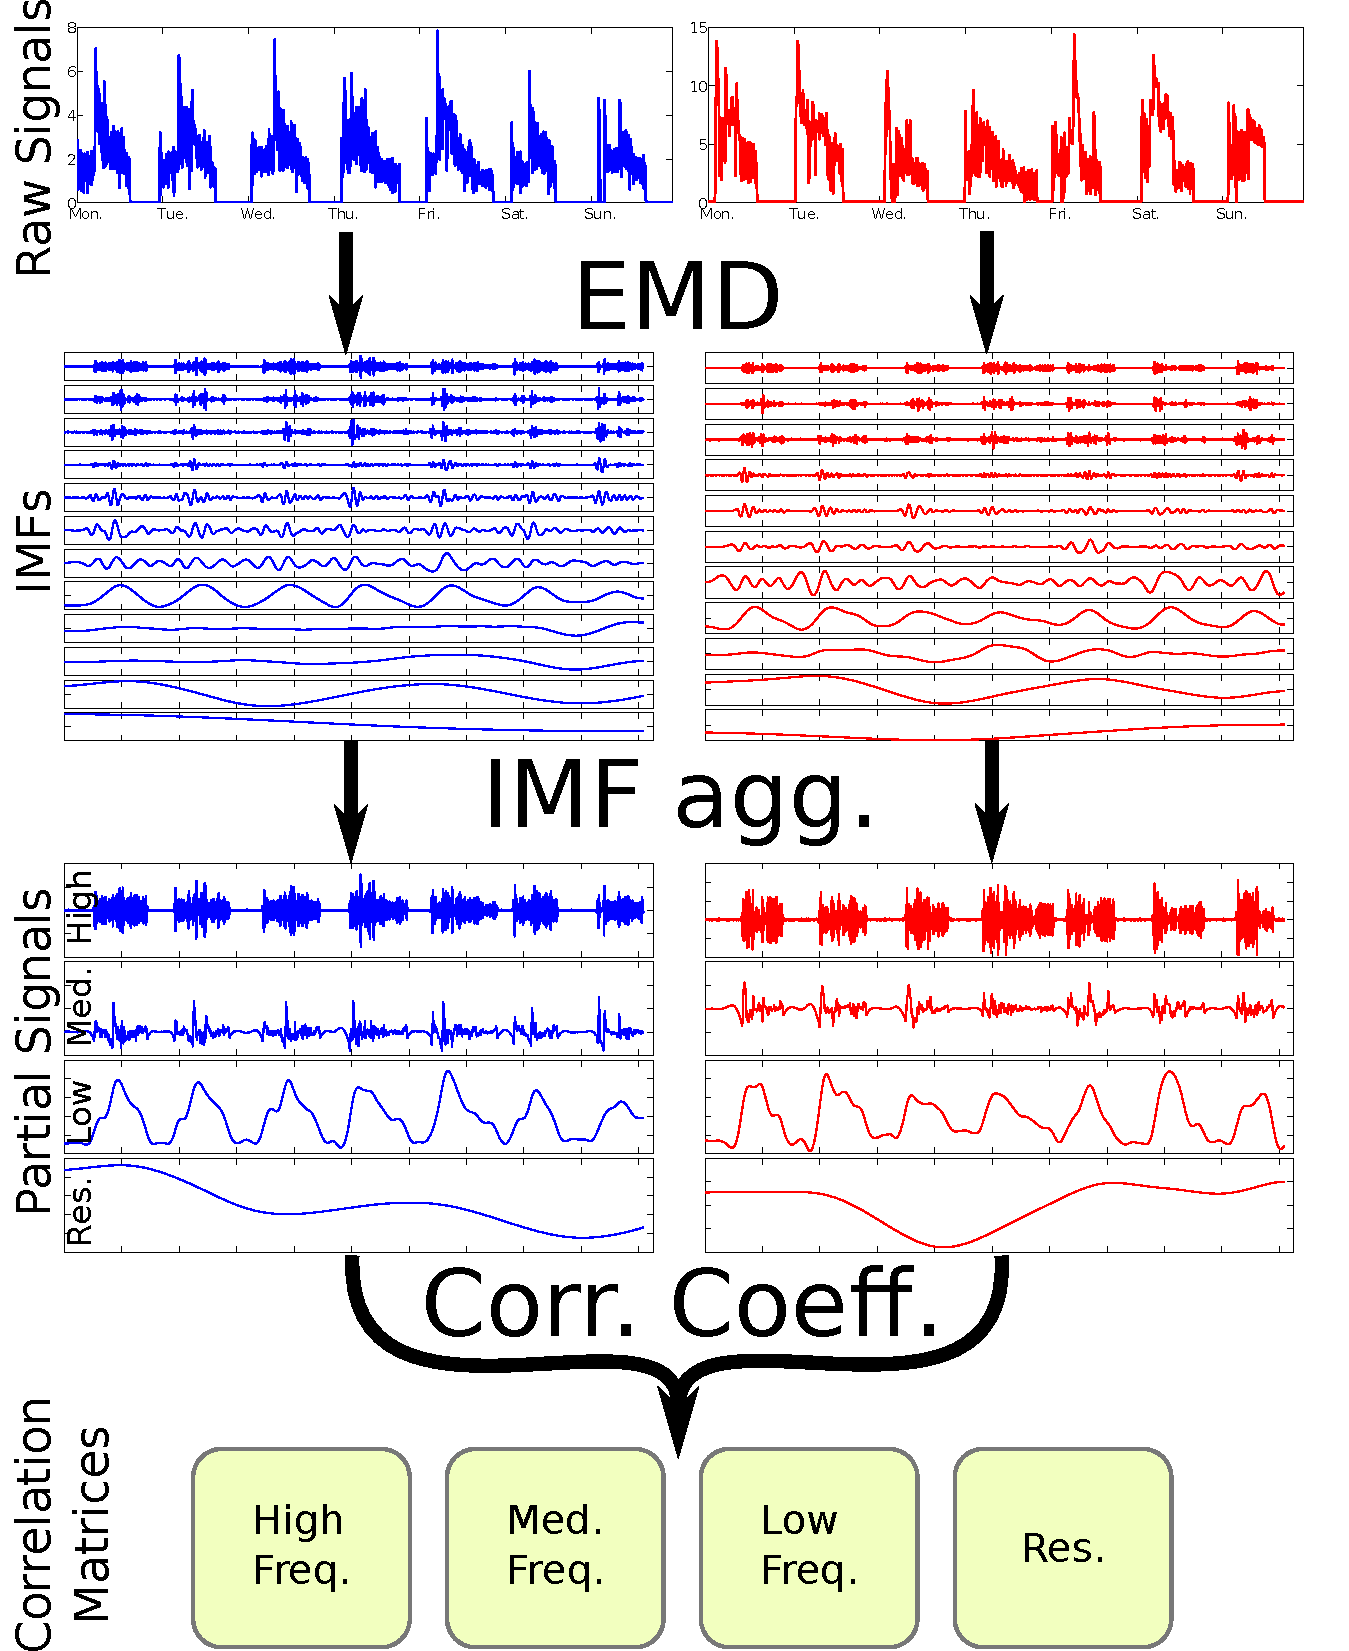
\includegraphics[width=.5\textwidth]{img/estimator.pdf}
 \caption{\emph{Strip and Bind} using two raw signals standing for one week of data from two different HVACs. (1)~Decomposition of the signals in IMFs using EMD (top to bottom: $c_1$ to $c_n$); (2)~aggregation of the IMFs based on their time scale; (3)~comparison of the partial signals (aggregated IMFs) using correlation coefficient.}
 \label{fig:diagram1}
\end{figure}

%As shown in the previous section, discovering the devices that are used in concert is particularly difficult.
Discovering devices that are used in concert is non-trivial.  
SBS decomposes each signal into an additive set of components, called Intrinsic Mode Functions (IMF), 
that reveals the signal patterns at different frequency bands.  IMFs are obtained using 
%that reveal the signal structures at different time scales.
Empirical Mode Decomposition (see Figure~\ref{fig:diagram1} and Section~\ref{emd}).
%Then, we filter out the IMFs that interfere with our goal and keep only those standing for time scales shorter than the unwanted daily pattern.
%We then remov out IMFs with time scales 
We only consider IMFs with time scales shorter than a day, since we are interested in capturing short-scale usage patterns.
Consequently, SBS aggregates the IMFs that fall into this specific time scale (see \emph{IMF agg.} in Figure \ref{fig:diagram1}).
%The resulting partial signals of different devices are compared pairwise to identify the devices intrinsic relationships (see \emph{Corr. Coeff.} in Figure\ref{fig:diagram1}). 
The resulting partial signals of different device power traces are compared, pairwise, to identify the devices that show un/correlated usage patterns (see \emph{Corr. Coeff.} in Figure~\ref{fig:diagram1}).


% These intrinsic relations are uncovered by comparing the sensors data at certain meaningful frequency bands.
% Namely, looking at high frequency allows to compare short-term variations representing the instantaneous devices change of state, however, the low frequency highlights long-term fluctuations revealing long devices usage pattern.
% 
% ..... the similarity estimators analyzes the readings from several sensors and reports scores standing for the similarity of the sensors at different frequency bands.
% First, the similarity estimator takes advantage of EMD to decompose the sensors signals into a set of components called intrinsic mode functions (IMFs).
% Second, it constructs band-limited signals by aggregating the IMFs whose mean frequencies fall in a certain frequency band.
% Thereby the pairwise comparison of band-limited signals provides the sensors correlations at different frequency bands. 
% 
% The advantages of the proposed intrinsic-correlation estimator are adaptive approach, ... 

% These two steps are described by the two following sections.

\subsubsection{Empirical Mode Decomposition} \label{emd}
Empirical Mode Decomposition (EMD) \cite{huang:emd1998} is a technique that decomposes a signal and reveals its intrinsic patterns, 
trend and noise.
This technique has been widely applied to a variety of datasets, including climate variables~\cite{lee:climateEMD2011}, medical data~\cite{blanco:bioMed2008}, speech signals~\cite{huang:signalProc2006,hasan:ieeeletter2009}, and image processing~\cite{nunes:vision2005}.
% for example, it helped to uncover the global surface temperature trends\cite{}, solar activity patterns and predicts climate variables .
EMD's effectiveness relies on its empirical, adaptive and intuitive approach.
In fact, this technique is designed to efficiently decompose both non-stationary and non-linear signals without requiring any 
a priori basis functions or tuning.  

EMD decomposes a signal into a set of oscillatory components called intrinsic mode functions (IMFs). 
An IMF satisfies two conditions: (1) it contains the same number of extrema and zero crossings (or differ at most by one); (2) the two 
IMF envelopes defined by its local maxima and local minima are symmetric with respect to zero.  Consequently, 
 IMFs are functions that directly convey the amplitude and frequency modulations.

% EMD is an iterative sifting process that extracts IMFs step by step; each step seeks for the IMF with the highest frequency, then the computed IMF is removed from the data and the residual data are used as input for the next step.
EMD is an iterative algorithm that extracts IMFs step by step by using the so-called sifting process \cite{huang:emd1998}; each step seeks for the IMF with the highest frequency by sifting, then the computed IMF is removed from the data and the residual data are used as input for the 
next step.
The process stops when the residual data becomes a monotonic function from which no more IMF can be extracted.

We formally describe the EMD algorithm as follows: 
\begin{enumerate}
\item Sifting process: For a current signal $h_0=X$, let $m_0$ be the mean of its upper and lower envelopes as determined from a cubic-spline interpolation of local maxima and minima.
\item The estimated local mean $m_0$ is removed from the signal, giving a first component: $h_1 = h_0-m_0$
\item The sifting process is iterated, $h_1$ taking the place of $h_0$. Using its upper and lower envelopes, a new local mean $m_1$ is computed and $h_2 = h_1-m_1$.
\item The procedure is repeated $k$ time until $h_k=h_{k-1}-m_{k-1}$ is an IMF according to the two conditions above.
\item This first IMF is designated as $c_1 = h_k$, and contains the component with shortest periods. We extract it from the signal to produce a residual: $r_1 = X - c_1$. The Steps 1 to 4 are iterated on the residual signal $r_1$, providing IMFs $c_j$ and residuals $r_j  = r_{j-1}-c_j$, for $j$ from $1$ to $n$.
\item The process stops when residual $r_n$ contains no more than 3 extrema.
\end{enumerate}

The result of EMD is a set of IMFs $c_i$ and the final residue $r_n$, such as: \[X=\sum^{n}_{i=1}c_i+r_n\]
where the size of the resulting set of IMFs $n$ depends on the original signal $X$ and $r_n$ represents the trend of 
the data (see \emph{IMFs} in Figure~\ref{fig:diagram1}).

For this work we implemented a variant of EMD called Complete Ensemble EMD~\cite{torres:icassp2012}.
This algorithm computes EMD several times with additional noise, it allows us to efficiently analyze signals that have 
flat sections (i.e. consuming no electricity in our case). % and permits us to solve the \emph{EMD mode mixing problem}.

\subsubsection{IMF aggregation} \label{methodo:corr}
By applying EMD to energy consumption signals we obtain a set of IMFs that precisely describe the devices consumption 
patterns at different frequency bands.  Therefore, we can focus our analysis on the smaller time scales, ignoring the dominant 
patterns that prevent us from effectively analyzing raw signals.

However, comparing the IMFs obtained from different signals is also not trivial,
 because EMD is empirically uncovering IMFs from the data there is no guarantee that the two IMFs $c_i^1$ and $c_i^2$ obtained from two distinct signals $S^1$ and $S^2$ represent data at the same frequency domain.
Directly comparing $c_i^1$ and $c_i^2$ is meaningless unless we confirm that they belong to the same frequency domain.

There are numerous techniques to retrieve IMF frequencies~\cite{huang:aada2009}.  
In this work we take advantage of the Generalized Zero Crossing (GZC)~\cite{huang:patent2006} because it is a simple and robust 
estimator of the IMF instantaneous frequency \cite{huang:aada2009}.
GZC is a direct estimation of IMF instantaneous frequency using critical points defined as the zero crossings and local extrema 
(round dots in Figure \ref{fig:gzc}).
Formally, given a data point $p$ GZC measures the quarter ($T_4$), the two halves ($T_2^x$) and the four full periods ($T_1^y$) $p$  belongs to (see Figure \ref{fig:gzc}) and the instantaneous period is computed as:
\[T=\frac{1}{7}\{4T_4+(2T_2^1+2T_2^2)+(T_1^1+T_1^2+T_1^3+T_1^4)\}\]

\begin{figure}
\begin{center}
 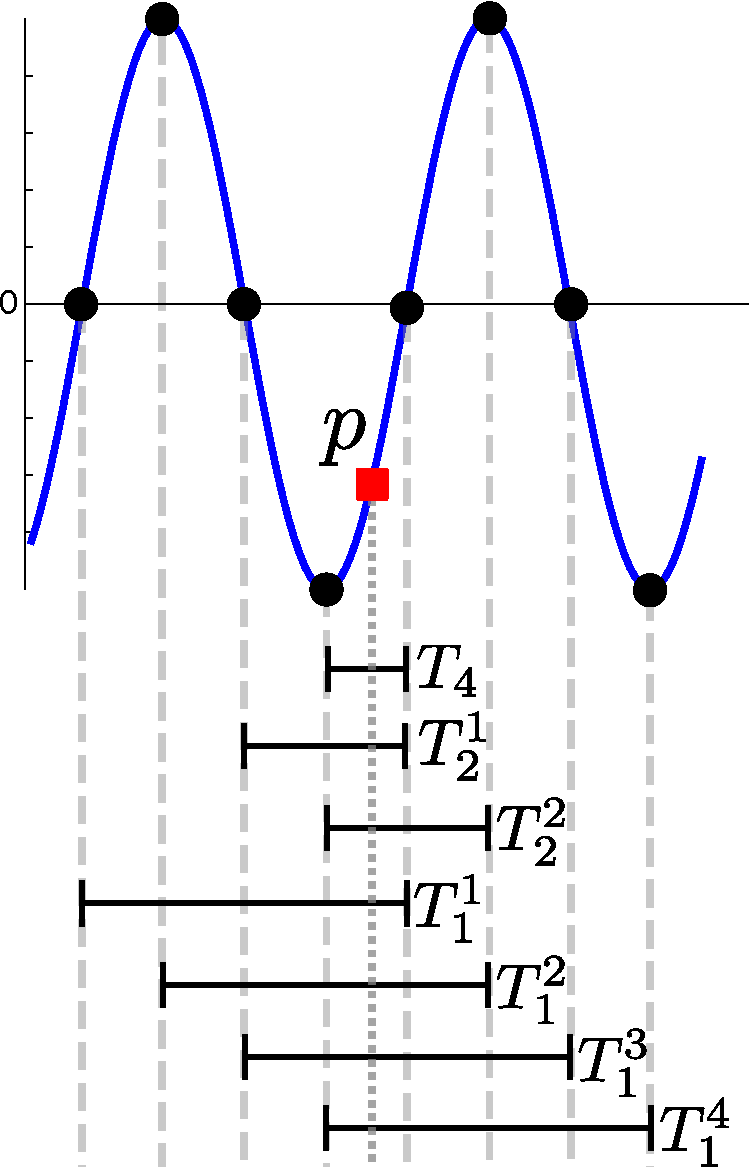
\includegraphics[width=.25\textwidth]{img/gzc.pdf}
 \end{center}
 \caption{Generalized Zero Crossing: the local mean period at the point $p$ is computed from one quarter period $T_4$, two half periods $T_2^x$ and four full periods $T_1^y$ (where $x=1, 2$, and, $y=1,2,3,4$).}
 \label{fig:gzc}
\end{figure}

Since all points $p$ between two critical points have the same instantaneous period GZC is local down to a quarter period.
Hereafter, we refer to the time scale of an IMF as the average of the instantaneous periods along the whole IMF.
Because the time scale of each IMF depends on the original signal, we propose the following to efficiently compare IMFs from different signals.
We cluster IMFs with respect to their time scales and partially reconstruct each signal by aggregating its IMFs from the 
same cluster.  Then, we directly compare the partial signals of different devices.

The IMFs are clustered using four time scale ranges: 
\begin{itemize}
 \item The \emph{high frequencies} stand for all the IMFs with a time scale lower than 20 minutes. These IMFs capture the noise.
 \item The \emph{medium frequencies} stand for all the IMFs with a time scale between 20 minutes and 6 hours. These IMFs convey the detailed devices usage.
 \item The \emph{low frequencies} stand for all the IMFs with a time scale between 6 hours and 6 days. These IMFs represent the daily pattern of the devices.
 \item The \emph{residual data} is all data with a time scale higher than 6 days. This is mainly the residual data obtained after applying EMD and it highlights the trend of the devices.
\end{itemize}

These time scale ranges are chosen based on our experiments and goal.
The 20-minute boundary relies on the sampling period of our dataset (5 minutes) and permits us to capture IMFs with really short periods.
The 6-hour boundary allows us to analyze all patterns that have a period shorter than the usual office hours.
The 6-day boundary allows us to capture daily patterns and weekday patterns.

Aggregating IMFs, within each time scale range, results in 4 partial signals representing different characteristics of the device's
 energy consumption (see \emph{Partial Signals} in Figure~\ref{fig:diagram1}).
We do a pairwise device trace comparison, calculating the correlation coefficient of their partial signals.
In the example shown in Figure~\ref{fig:diagram1}, the correlation coefficient of the raw signals suggests that they are highly correlated ($0.57$). 
However, the comparison of the corresponding \emph{partial signals} provides new insights;
the two devices are poorly correlated at high and medium frequencies (respectively $-0.01$ and $-0.04$) but highly correlated at low frequencies ($0.79$) meaning that these devices are not ``intrinsically'' correlated.  They only share a similar daily pattern.

All the devices are compared pairwise at the four different time scale ranges.
Consequently, we obtain four correlation matrices that convey the device similarities at different time scales.
Each line of these matrices (or column, since the matrices are symmetric) reveals the behavior of a device -- its relationships with the 
other devices at a particular time scale.
The matrices form the basis for tracking the behavior of devices and to search for misbehavior.


\subsection{Search}\label{methodo:ano}
\emph{Search} aims at identifying misbehaving devices in an unsupervised manner.
Device behavior is monitored via the correlation matrices presented in the previous section.
Using numerous observations SBS computes a specific reference that exhibits the normal inter-device usage pattern.
Then, SBS compares the computed reference with the current data and reports devices that deviate from their usual 
behavior.

\subsubsection{Reference}
We define four reference matrices, which capture normal device behavior at the four time scale ranges defined in 
Section~\ref{methodo:corr}.
The references are computed as follows: (1) we retrieve the correlation matrices for $n$ consecutive time bins (as described in Section~\ref{methodo:est}). (2) For each pair of devices we compute the median correlation 
over the $n$ time bins and obtain a matrix of the median device correlations.

Formally, for each time scale range the computed reference matrix for $d$ devices and $n$ time bins is:
\[R_{i,j} =  \median(C^1_{i,j},...,C^n_{i,j})\]
where $i$ and $j$ ranges in $[1,d]$.

% Assuming that device-usage predominantly behaves normally and the anomalies are exceptional 
% events, the reference matrices exhibit the normal device behaviors.
Our model assumes anomalies are rare and the majority of the data is normal.
This is a common assumption in unsupervised anomaly detection.
% We assume that normal behavior is not truly anomalous.
Abnormal correlation values, that could appear during model construction, %in the analyzed time bins 
are ignored by the median operator thanks to its robustness to outliers (50\% breakdown point).  
However, if that assumption does not hold (more than 50\% of the data is anomalous), our model will flag the opposite -- labeling abnormal as normal and vice-versa.
From close inspection of our data, we believe our primary assumption is sound.
% Normal behavior occurs most frequently, therefore detected anomalies should be meaningful.



\subsubsection{Behavior change}
% SBS consists in identifying the devices that significantly deviate from their normal behaviors as defined in the reference matrices.
% Consequently, 
We compare each device behavior, for all time bins, to the one provided by the reference matrix.  
Consider the correlation matrix $C^t$ obtained from the data for time bin $t$ ($1 \leq t \leq n$).  
Vector $C^t_{i,*}$ is the behavior of the $i^{th}$ device for this time bin.
Its normal behavior is given by the corresponding vector in the reference matrix $R_{i,*}$.
We measure the device behavior change at the time bin $t$ with the following Minkowski weighted distance:
\[ l^t_{i} = \left(\sum_{j=1}^d  w_{ij}\left(C^t_{i,j} - R_{i,j}\right)^p\right)^{1/p} \]
where $d$ is the number of devices and $w_{ij}$ is:
\[ w_{ij} = \frac{R_{i,j}}{\sum_{k=1}^d R_{i,k}}. \]
The weight $w$ enables us to highlight the relationship changes between the device $i$ and those highly correlated to it in the reference matrix.
In other words, our definition of behavior change is mainly driven by the relationship among devices that are usually used in concert.
We also set $p=4$ in order to inhibit small differences between $C^t_{i,j}$ and $R_{i,j}$ but emphasize the important ones.

By monitoring this quantity over several time bins the abnormal device behaviors are easily identified as the outlier values.
In order to identify these outlier values we implement a robust detector based on median absolute deviation (MAD), a dispersion measure commonly used in anomaly detection \cite{huber:wiley2009,chan:springer2005}.
It is a measure that robustly estimates the variability of the data by computing the median of the absolute deviations from the median of the data.
 Let $l_{i} = [l_i^1,...,l_i^n]$ be a vector representing the behavior changes of device $i$ over $n$ time bins, then its MAD value is defined as:
\[ \mad_i = b \median(\lvert l_{i} - \median(l_{i})\rvert)\]
where the constant $b$ is usually set to $1.4826$ for consistency with the usual parameter $\sigma$ for Gaussian distributions.
Consequently, we define anomalous behavior, for device $i$ at time $t$, such that the following equation is satisfied:%of the device $i$ at the time bin $t$ that satisfies the following equation:
\[l^t_{i} > \median(l_{i}) + \tau  \mad_i\]
Note, $\tau$ is a parameter that permits to make SBS more or less sensitive.

The final output of SBS is a list of alarms in the form $(t,i)$ meaning that the device $i$ has abnormal behavior at the time bin $t$.
The priority of the alarms in this list is selected by the building administrator by tuning the parameter $\tau$.


\section{Data sets}
We evaluate SBS using data collected from buildings in two different geographic locations.  
%One is a recent building at the University of Tokyo main campus and the other one is another building at the University of California Berkeley.

\subsection{Building 1} \label{data:engbldg2}
%The data from building 1 is collected at the Engineering Building 2 of the Hongo campus. 
Building 1, is a 12-story building completed in 2005 and is now hosting classrooms, laboratories, professor offices 
and server rooms.  In addion, rather than a centralized HVAC system, small, local HVAC system are set up throughout
the buidling.  The electricity consumption of the lighting and HVAC systems of 231 rooms is monitored by 135 sensors.
The HVAC system of this building is decentralized and the corresponding devices are classified into two categories, EHP (Electrical Heat Pump) 
and GHP (Gas Heat Pump).
The GHPs are the only devices that serve numerous rooms on several floors.  The 5 GHPs of the dataset serve 154 rooms.
The EHP and lighting systems serve only pairs of rooms and they are independently controlled by the rooms users.
In addition, metadata associated to each sensor provides the type of the monitored device and the associated room number, 
therefore, the electricity consumption of each pair of rooms is separately monitored.

The dataset contains 10 weeks of data starting from June $27^{th}$ 2011 and ending on September $5^{th}$ 2011.
This period of time is particularly interesting for two reasons; in this region, the summer is the most energy-demanding 
season and the building manager actively works to curtail energy usage as much as possible.
%, and at that time the university has initiated several power-saving measures due to the the Tohoku earthquake and Fukushima nuclear accident.

Furthermore, this dataset is a valuable ground truth to evaluate the Strip and Bind part of SBS.
Since the light and HVAC of the rooms are directly controlled by the room's occupants, we expect SBS to uncover verifiable devices 
relationships.  
% In addition, we expect the anomaly detector to identify discontinuities in these relationships that represent obvious electricity saving opportunities (e.g. a room HVAC left on during night while the room lights have been turned off).

% Due to privacy concern this dataset is not publicly available on the Internet but accessible upon request.

\subsection{Building 2}
Building 2 is a 5-story building hosting mainly classrooms, meeting rooms, laboratories and a datacenter.
This building was completed in 1950, thus its infrastructure is significantly different from the one of the Building 1.
The HVAC system in the building is centralized and serves couple of floors per unit.
There is a separate unit for an internal fabricated laboratory, inside the building.
%Nevertheless, we notice an independent HVAC system that was serving a particular laboratory; the Microfabrication Laboratory (Microlab).

This dataset consists of 8 weeks of energy consumption traces measured by 70 sensors from April $5^{th}$ 2011.
Contrary to the other dataset, a variety of devices are monitored, including, receptacles on certain floors, most of the HVAC components, 
 power panels for different floors and the whole building consumption.

Analyzing these two datasets is particularly appealing because the two building infrastructures are fundamentally different. 
This enables us to evaluate the practical efficacy of the proposed, unsupervised method in two different environments.


\subsection{Data pre-processing}
Elaborated data pre-processing is not required for the proposed approach.
Nevertheless, we observed in a few exceptional cases that sensors reporting excessively high values (i.e. values higher than the device actual capacity) greatly alter the performance of the proposed method.
Because these values are outstanding in the corresponding signal they bias the computation of the correlation coefficient.
Therefore, we remove from the raw signal values that are higher than the maximum capacity of the device.

In addition, to compare signals of the same length, the raw data is arranged such that the energy consumption of each device is reported every 5 minutes. 



\begin{figure*}[t!]
% \subfloat[Raw signals]{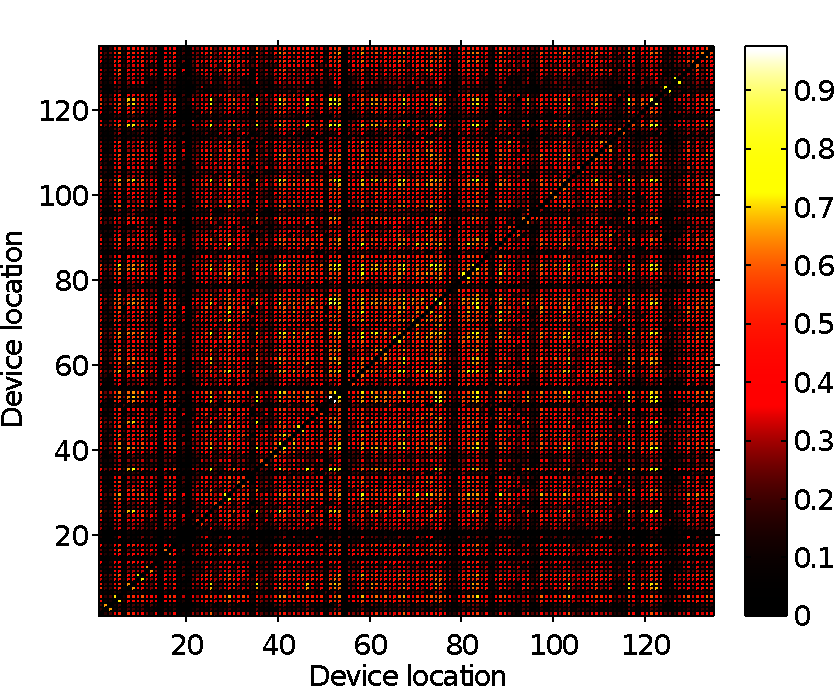
\includegraphics[width=.48\textwidth]{img/heatMap_raw_201106-eps-converted-to.pdf}}\\
\subfloat[High Frequencies\label{fig:heatmap:high}]{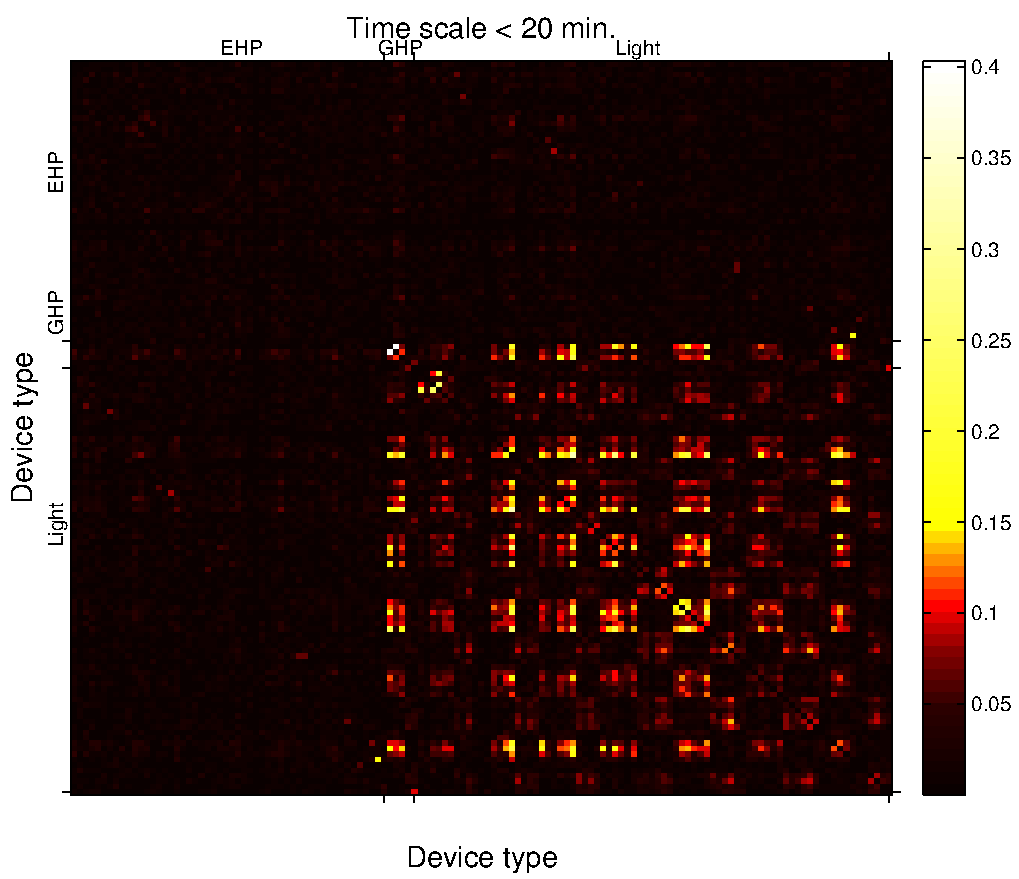
\includegraphics[width=.48\textwidth]{img/heatMap_1_201106-eps-converted-to.pdf}}\hfill
\subfloat[Medium Frequencies\label{fig:heatmap:med}]{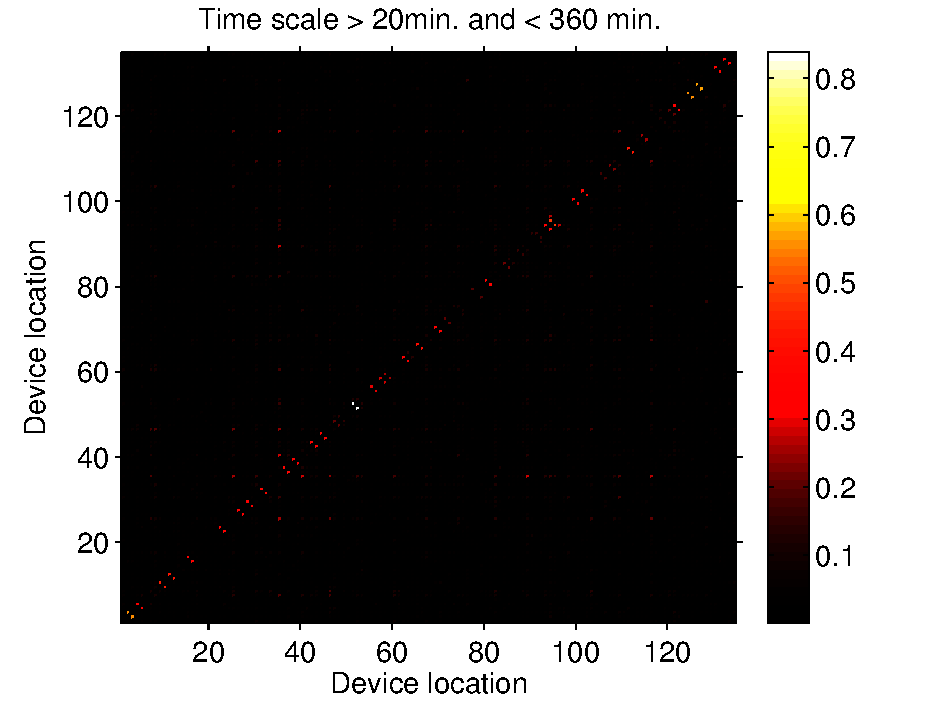
\includegraphics[width=.48\textwidth]{img/heatMap_2_201106-eps-converted-to.pdf}}\\
\subfloat[Low Frequencies\label{fig:heatmap:low}]{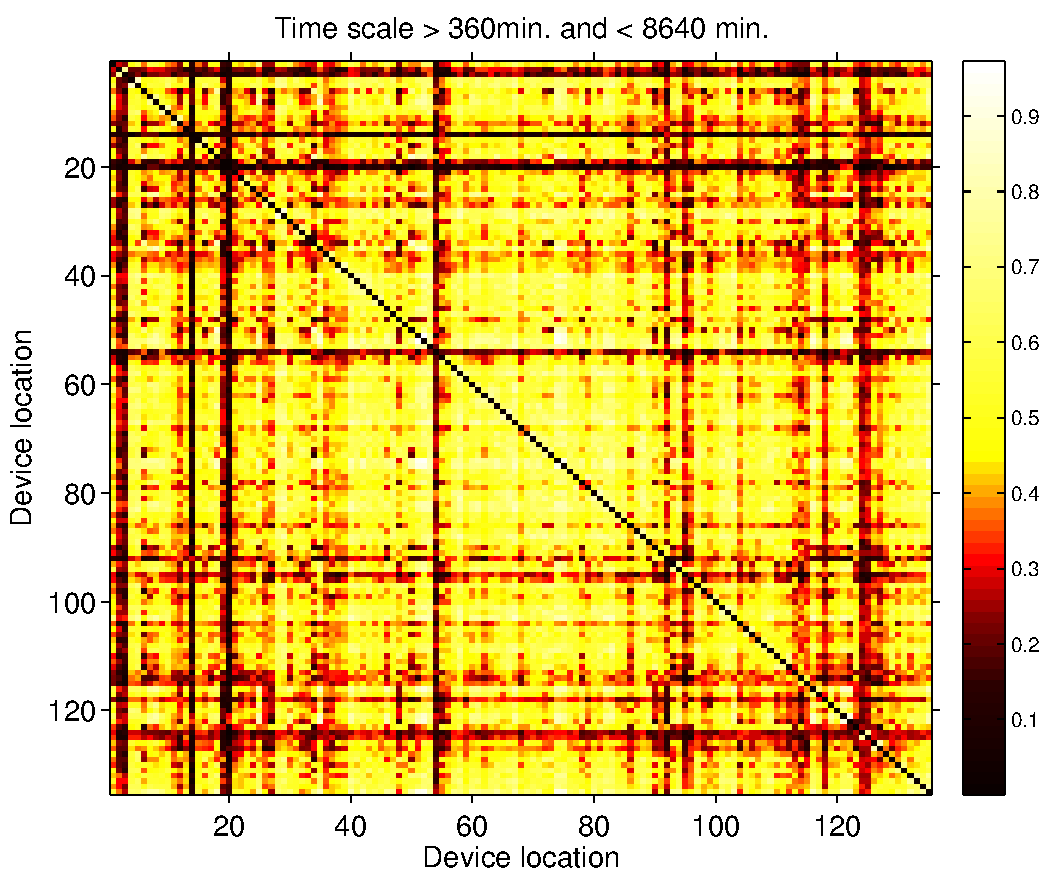
\includegraphics[width=.48\textwidth]{img/heatMap_3_201106-eps-converted-to.pdf}}\hfill
\subfloat[Residual data\label{fig:heatmap:res}]{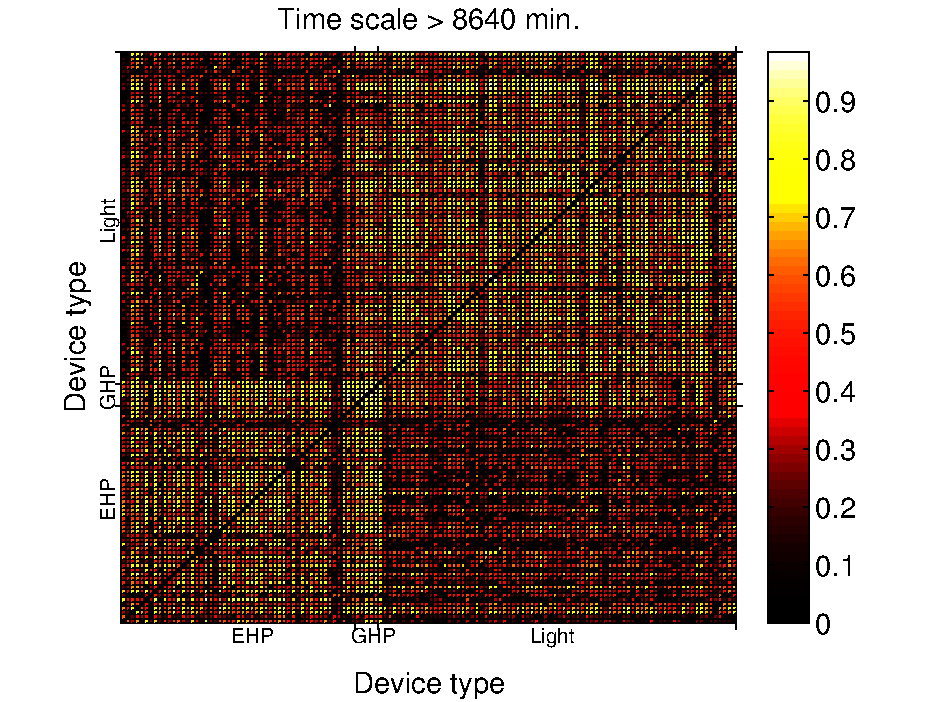
\includegraphics[width=.48\textwidth]{img/heatMap_4_201106-eps-converted-to.pdf}}
\caption{Reference matrices for the four time scale ranges (the diagonal $x=y$ is colored in black for better reading). The medium frequencies highlight devices that are located next to each other thus intrinsically related. The low frequencies contains the common daily pattern of the data. The residual data permits to visually identify devices of the similar type.}
\label{fig:heatmap}
\end{figure*}

\section{Experimental Results}
\label{eval}
In this section we evaluate SBS on our building traces.  We demonstrate
 the benefits of striping the data by monitoring patterns captured at different time scales.
Then, we thoroughly investigate the alarms reported by SBS.  

\subsection{Shortingcomings}
Because our analysis is done on historical data, some of the faults found by SBS could not be fully
corroborated.  In order to fully examine the effectiveness of our approach, we must run it in real time and
physically check that the problem is actually occurring.  When a problem is detected
in the historical trace, months after it has occurred, the current state of the building may no longer reflect
what is in the traces.  Some of the anomalies discussed in this section uncover interpretable patterns 
that are difficult to find in practice.  For example, simultaneous heating and cooling is a known, recurring problem
 in buildings, but it is very hard to identify  when it is occurring.  Some of the anomalies we could not interpret
might be interpretable by a building manager, however, we did not consult either building manager for this study.
The results of this study, therefore, do not exmaine the true/false positive rate for this reason.

The true/false negative rate is impractical to assess.  It may be examined through synthetic stimulation of
the building via the control system.  However, getting cooperation from a building manager to hand over control of the building
for experimentation in non-trivial.  Therefore, we forgo a full true/false negative analysis in our evaluation.

Because of these challenges, the evaluation of SBS focuses on comparing the output with known fault
signatures.  We examine anomalies, in either buildings, where the anomaly is easily interprettable but
difficult to find by the building manager.  We forego a comparison of SBS with competing algorithms because
 related algorithms require detailed knowledge of the building, \emph{a priori}.  The advantage of SBS is that it 
 does not require any such information provide immediate value.

\subsection{Device behavior at different time scales}
The Strip and Bind part of SBS is evaluated using the data from the Building 1. %, since we can verify how items are being used and use it as ground truth.
This dataset is appropriate to measure SBS's performance, since lighting and HVAC systems serving the same room are usually used 
simultaneously.
Consequently, we analyze this data using SBS and verify that the higher correlations at medium frequencies correspond to devices located in the same room. % and the unwanted data is captured at the other frequencies.

The dataset is split in 10 bins of 1 week long and each bin is processed by SBS.
Using the 10 correlation matrices at each time scale range SBS uncovers the four reference matrices depicted in 
Figure \ref{fig:heatmap}.

\paragraph{High frequencies}
In this work the high frequencies correspond to the signals \emph{noise}, 
therefore, we do not expect any useful information from the corresponding matrix (Figure \ref{fig:heatmap:high}).
Indeed, the corresponding reference matrix does not provide any help to determine a device's relative location.
Thus, we emphasize that high frequency data should be ignored for uncovering device relationships (in contrast to \cite{romain:iotapp12}).
Interestingly, we find that the sensors monitoring the lights generate consistent noise. % and could help one to cluster this type of sensor.
  
\paragraph{Medium frequencies}
Our main focus is on the medium frequencies as it is designed to capture the intrinsic device relationships.
Figure \ref{fig:heatmap:med} shows the correlation matrix at medium frequencies.
It is significantly different from the one obtained with the raw signals (Figure \ref{fig:heatmap:raw}): high correlation coefficients are concentrated along the matrix diagonal. 
Since devices serving the same or adjacent rooms are placed nearby in the matrix it validates our hypothesis: \emph{high correlation scores within the medium frequency band shows strong inter-device relationships}.

Considering this reference matrix as an adjacency matrix of a graph, in which the nodes are the devices, we identify the clusters of 
correlated devices using a community mining algorithm~\cite{blondel:unfolding}.
As expected we obtain mainly clusters of only two devices (light and HVAC serving the same room), but we also find clusters that are composed of more devices.
For example a cluster contains 3 HVAC systems serving the three server rooms. Although these server rooms are located on
 different floors, SBS shows a strong correlation between these devices.  Coincidentally, they are managed similarly.
Interestingly, we also observe a couple of clusters that consist of independent devices serving adjacent rooms belonging to the same lab.
The bigger cluster contains 33 devices that are 2 GHP devices and the corresponding lights.
This correlation matrix and the corresponding clusters 
highlight the ability for SBS to identify such hidden inter-device usage relationships.
 
\paragraph{Low frequencies}
Low frequencies capture daily patterns, embedded in all the device traces.  
Figure \ref{fig:heatmap:low} depicts the corresponding reference matrix which is similar to the one of raw signal traces (Figure \ref{fig:heatmap:raw}) 
and it shows no particular structure.% (daily patterns account for the coefficients high values).
% Since this matrix contains mainly high values, most of the partial signals at low frequencies features similar characteristics (i.e. daily patterns).
These partial signals are discarded as they do not help us in identifying inter-device usage patterns.
 
\paragraph{Residual data}
The residual data shows the weekly trend, which gives us no information about device relationships.
But, surprisingly, by reordering the correlation matrix based on the type of the devices (Figure \ref{fig:heatmap:res}) 
we can visually identify two major clusters.
The first cluster consists of HVAC devices (see EHP and GHP in Figure \ref{fig:heatmap:res}) and the second one contains only lights. 
An in-depth examination of the data reveals that long-term trends are inherent to the device types. 
For example, as the consumption of both the EHP and GHP devices is driven by the building occupancy and the outside temperature, these two types of devices follow the same trend. 
However, the use of light is independent from the outside temperature thus the lighting systems follow a common trend different from the EHP and GHP one.

We conduct the same experiments by splitting the dataset in 70 bins of 1 day long and observe analogous results at high and medium frequencies but not at lower frequencies.  This is because the bins are too short to exhibit daily oscillations and the residual data captures only the daily trend.

% TODO add some info about the reference matrix for the Building 2?

\subsection{Anomalies}
We now evaluate the \emph{search} performance of SBS using the traces from the Building 1 and the Building 2.
%% Romain
Due to the lack of historical data, such as room schedule or reports of energy waste, this evaluation is non trivial.
Furthermore, getting ground truth data from a manual inspection of the hundreds traces of our data sets is impractical.
The lack of ground truth data prevents us from producing a systematic analysis of the anomalies missed by SBS (i.e. false negatives rate).
Nevertheless, we exhibit the relevance of the anomalies uncovered by SBS (i.e. high true positive rate and low false positive rate) by manually checking the output of SBS.
%% Romain

\paragraph{Anomaly classification}
To validate SBS results we manually inspect the anomalies detected by the algorithm.  
For each reported alarm $(t,i)$ we investigate the device trace $i$ and the devices correlated to it
to determine the reason for the alarm.
Specifically, we retrieve the major relationship change that causes the alarm (i.e. $\max(|w_j(C_{i,j}^t - R_{i,j})|)$, 
see Section \ref{methodo:ano}) and examine the metadata associated to the corresponding device.
% $j$ and the sign of the relationship change $C_{i,j}^t - R_{i,j}$.
% A positive value of relation change means the devices correlation at the time bin $t$ is abnormally high, whereas negative value means that the relationship between the two devices is broken.
This investigation allows us to classify the alarms into five groups:
\begin{itemize}
 \item \emph{High power usage}: alarms corresponding to electricity waste.
 \item \emph{Low power usage}: alarms representing the abnormally low electricity consumption of a device.
 \item \emph{Punctual abnormal usage}: alarms standing for short term (less than 2.5 hours) raise or drop of the electricity consumption.
 \item \emph{Missing data}: alarms raised due to a sensor failure.
 \item \emph{Other}: alarms whose root cause is unclear.
\end{itemize}

% However, the exhaustive enumeration of the true negatives (i.e. saving opportunities that are not detected) is impractical because of the size of the analyzed datasets (number of devices and traces length).
% Instead we exhibit the detector sensitivity by varying $\tau$, the threshold value.

\begin{figure}
\begin{center}
 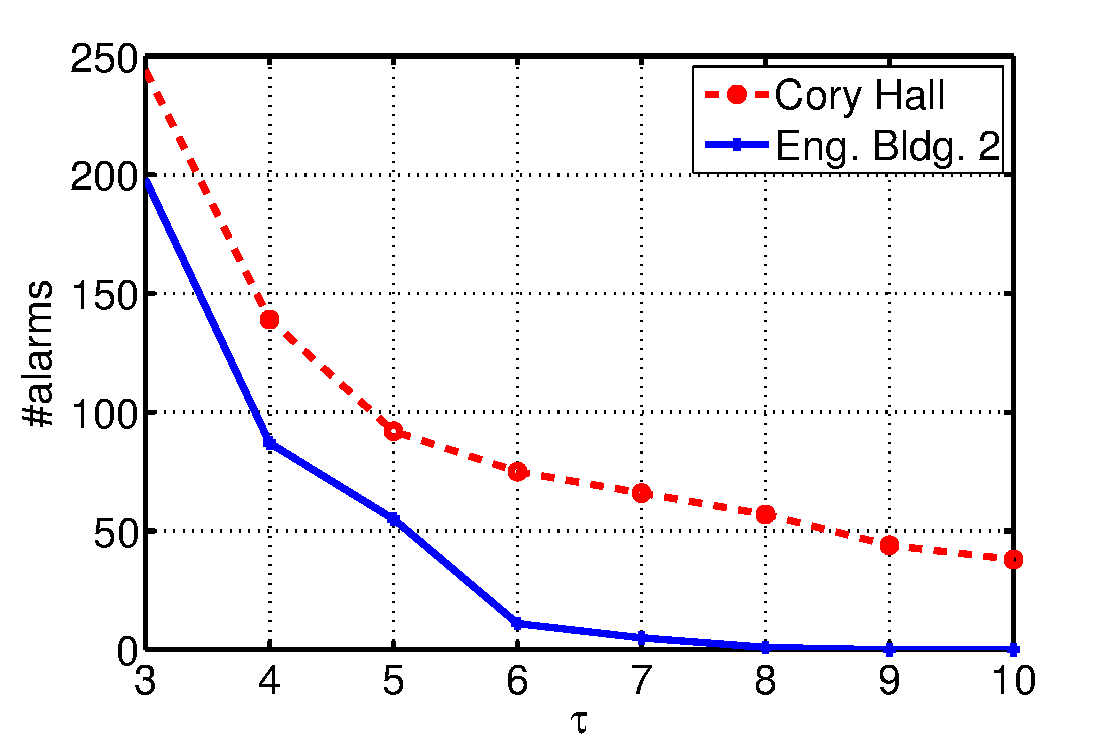
\includegraphics[width=.49\textwidth]{img/threshold-eps-converted-to.pdf}
 \caption{Number of reported alarms for various threshold value ($\tau=[3,10]$).}
 \label{fig:thres}
 \end{center}
\end{figure}

\begin{table}
\begin{center}
\begin{tabular}{|l||c|c|c|c|c|}
\hline
&High&Low&Punc.&Missing&Other\\ \hline \hline
Building 1& 9 (5) & 6 (5) & 1 (1) & 36 (1) & 3 (3) \\ \hline
Building 2& 25 (7) & 7 (3) & 4 (4) & 0 (0) & 3 (3) \\ \hline
\end{tabular}
\end{center}
\caption{Classification of the alarms reported by SBS for both dataset (and the number of corresponding anomalies).}
\label{tab:classif}
\end{table}

\paragraph{Experimental setup}
For each experiment, the data is split in time bins of one day, starting from 09:00 a.m. -- which is approximately 
the office's opening time.
We avoid having bins start at midnight since numerous anomalies appear at night and they are better highlighted if they are 
not spanning two time bins.
Only the data at medium frequencies are analyzed, the other frequency bands are ignored.


The threshold $\tau$ tunes the sensitivity of SBS, hence, the number of reported alarms.  
Furthermore, by plotting the number of alarms against the value of $\tau$ for both datasets (Figure \ref{fig:thres}) we observe an 
elbow in the graph around $\tau=5$.
With thresholds lower than this pivot value ($\tau<5$), the number of alarms significantly increases, causing less important anomalies 
to be reported.  
For higher values ($\tau>5$), the number of alarms is slowly decreasing, providing more conservative results that consist of the 
most important anomalies.
This pivot value provides a good trade off for either data set.

\begin{figure*}
  \subfloat[High power usage where the HVAC (EHP) is turned on at night\label{fig:res:eng1}]{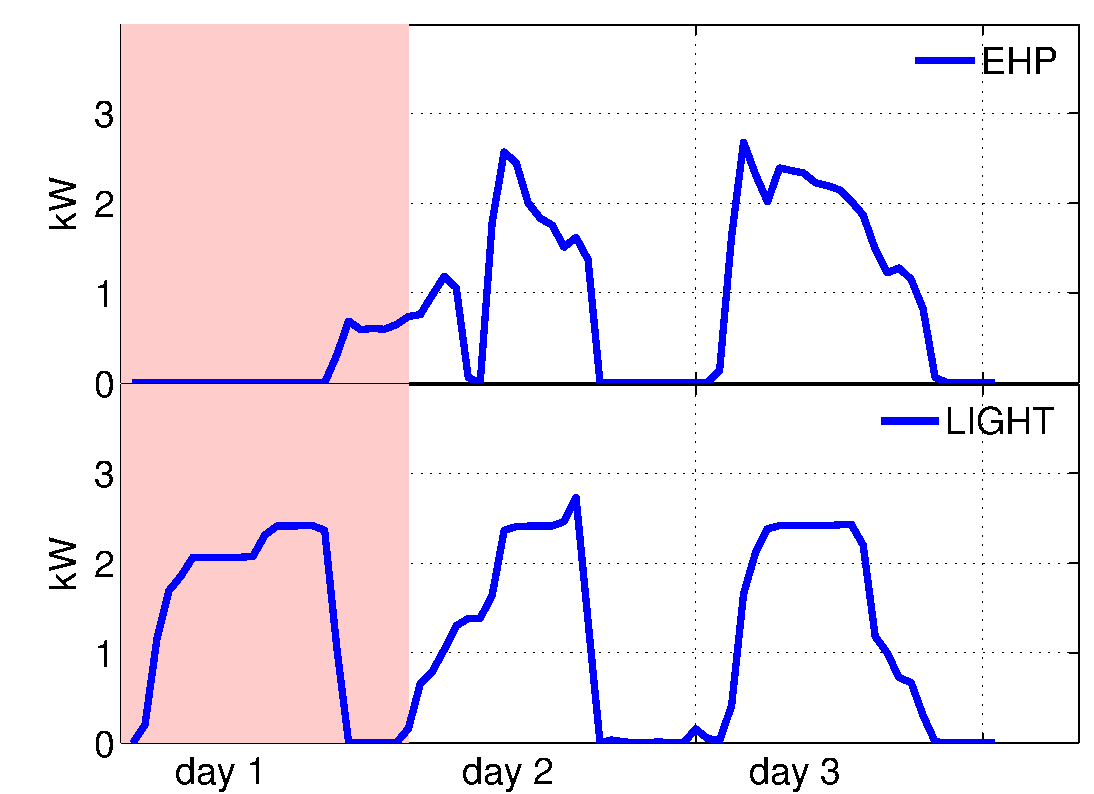
\includegraphics[width=.32\textwidth]{img/0sig20_sig31alarm1-eps-converted-to.pdf}} \hspace{.015\textwidth} %EHP turned on at night!?
  \subfloat[High power usage where the light is left on at night\label{fig:res:eng2}]{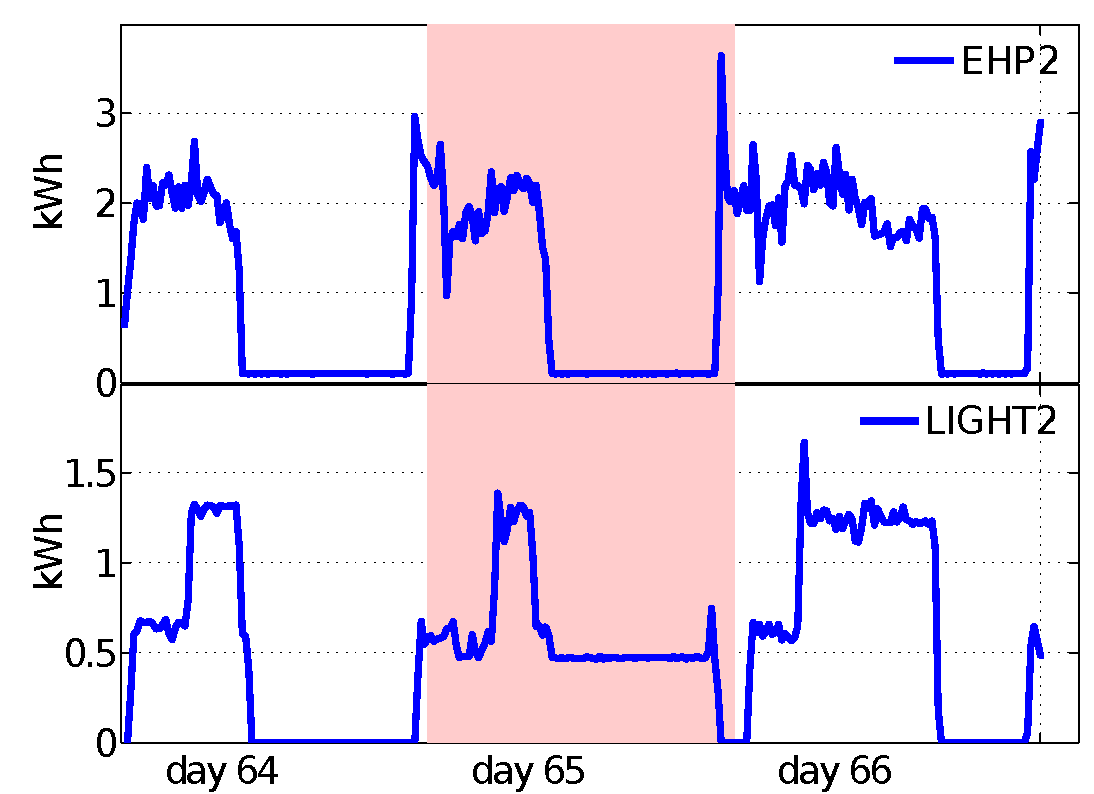
\includegraphics[width=.32\textwidth]{img/0sig123_sig134alarm65-eps-converted-to.pdf}} \hspace{.015\textwidth}  %Light left on during night
 \subfloat[Low power usage where the HVAC (EHP) is not used during office hours\label{fig:res:eng3}]{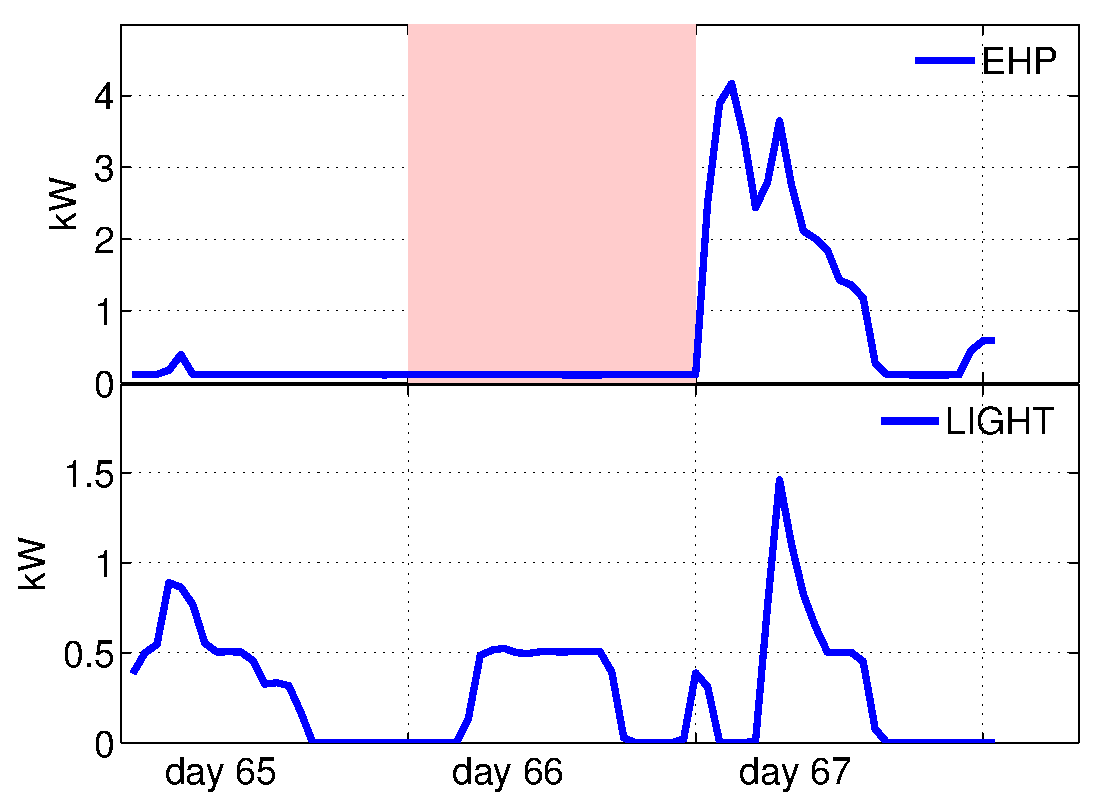
\includegraphics[width=.32\textwidth]{img/0sig24_sig33alarm66-eps-converted-to.pdf}}\\ %Three EHPs that are really correlated
 \subfloat[Long term high power usage partially detected\label{fig:res:eng4}]{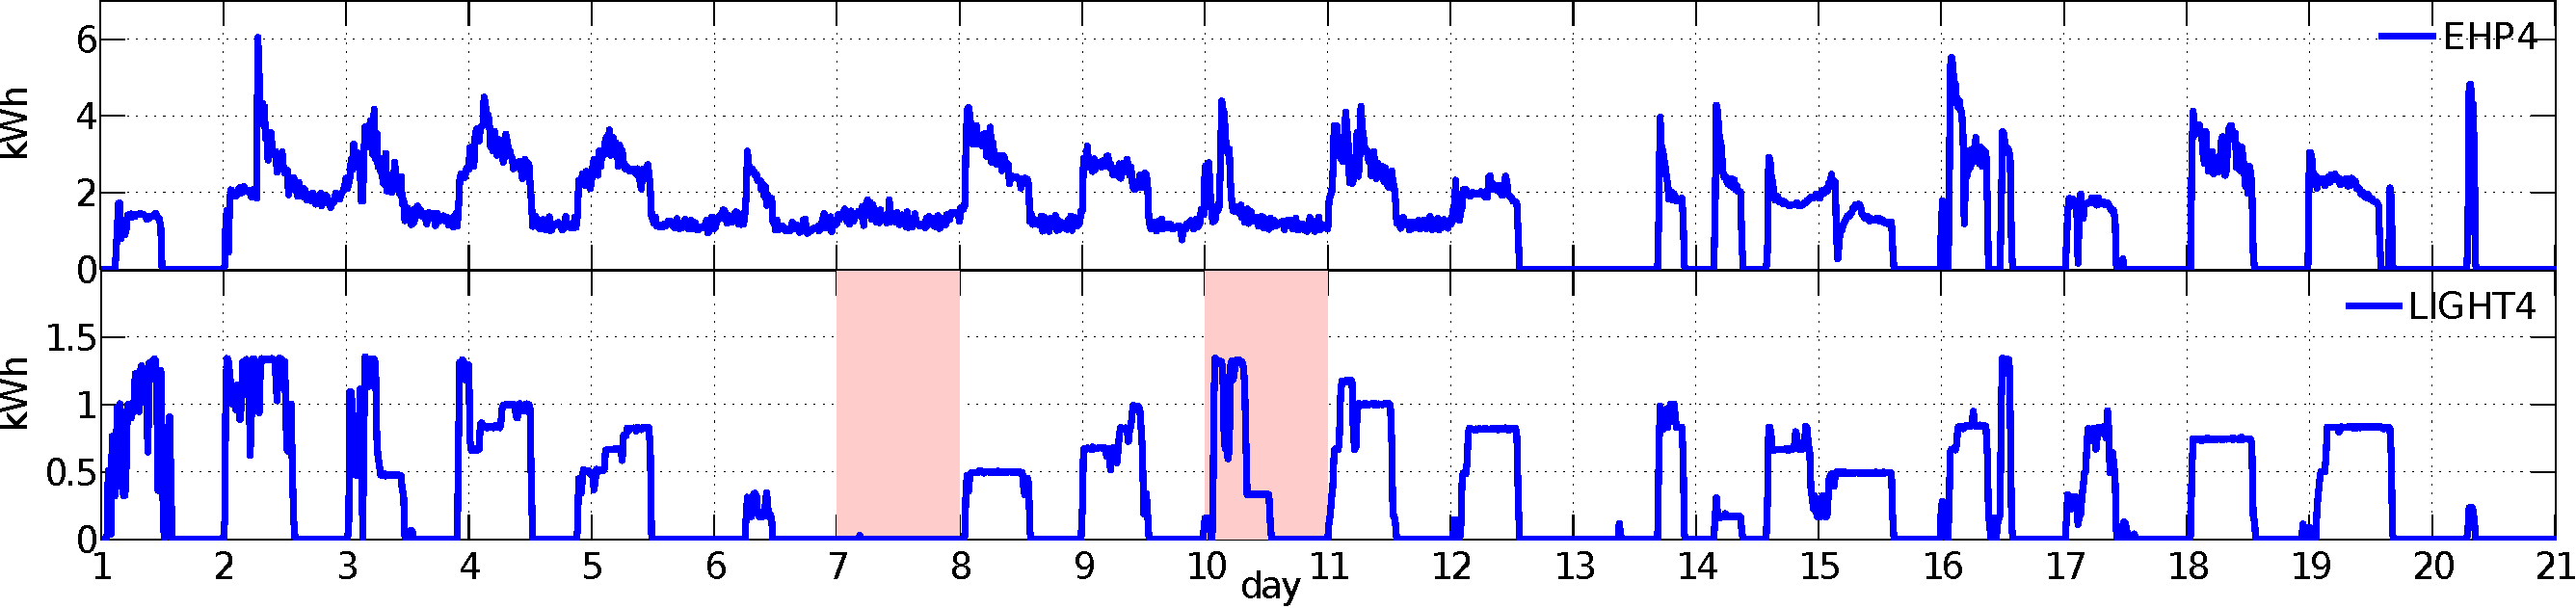
\includegraphics[width=\textwidth]{img/0sig3_sig15alarm7-eps-converted-to.pdf}}\\  
\caption{Example of alarms (red rectangles) reported by SBS on the Building 1 dataset}
\end{figure*}


Table \ref{tab:classif} classifies the alarms reported by SBS on both datasets.
 Anomalies spanning several time bins (or involving several devices) may raise several alarms.  We display these in Table \ref{tab:classif} 
 as numbers in brackets -- the number of anomalies corresponding to the reported alarms.
%Due to page limitation the following sections only present the most typical and interesting anomalies identified by SBS.

\subsubsection{Building 1}


SBS reported 55 alarms over the 10 weeks of the Building 1 dataset.
However, 36 alarms are set aside because of sensor errors; one GHP has missing data for the first 18 days.
Since this device is highly correlated to the GHP in the reference matrix, their relationship is broken for the 18 first bins and 
for each bin one alarm per device is raised.

\begin{figure*}
  \subfloat[Low power usage due to a chiller failure\label{fig:res:cory1}]{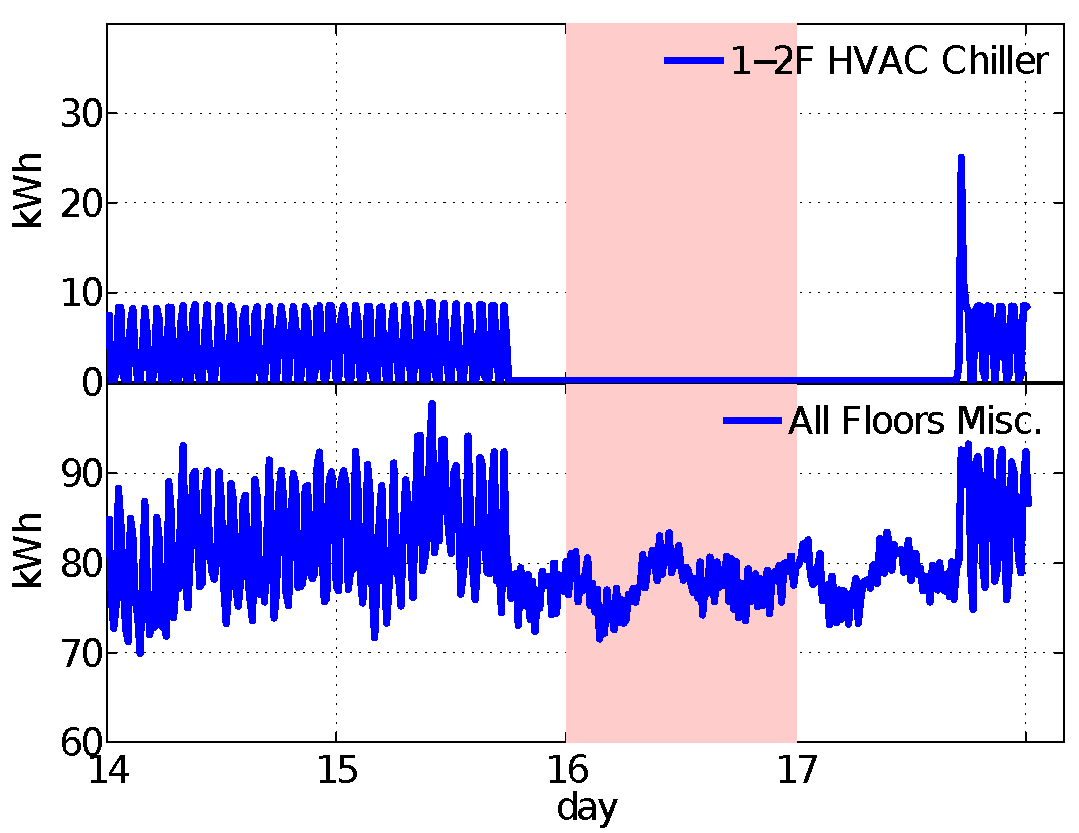
\includegraphics[width=.32\textwidth]{img/1sig37_sig55alarm16-eps-converted-to.pdf}} \hspace{.015\textwidth}
 \subfloat[High power usage highlighted by the elevator usage\label{fig:res:cory21}]{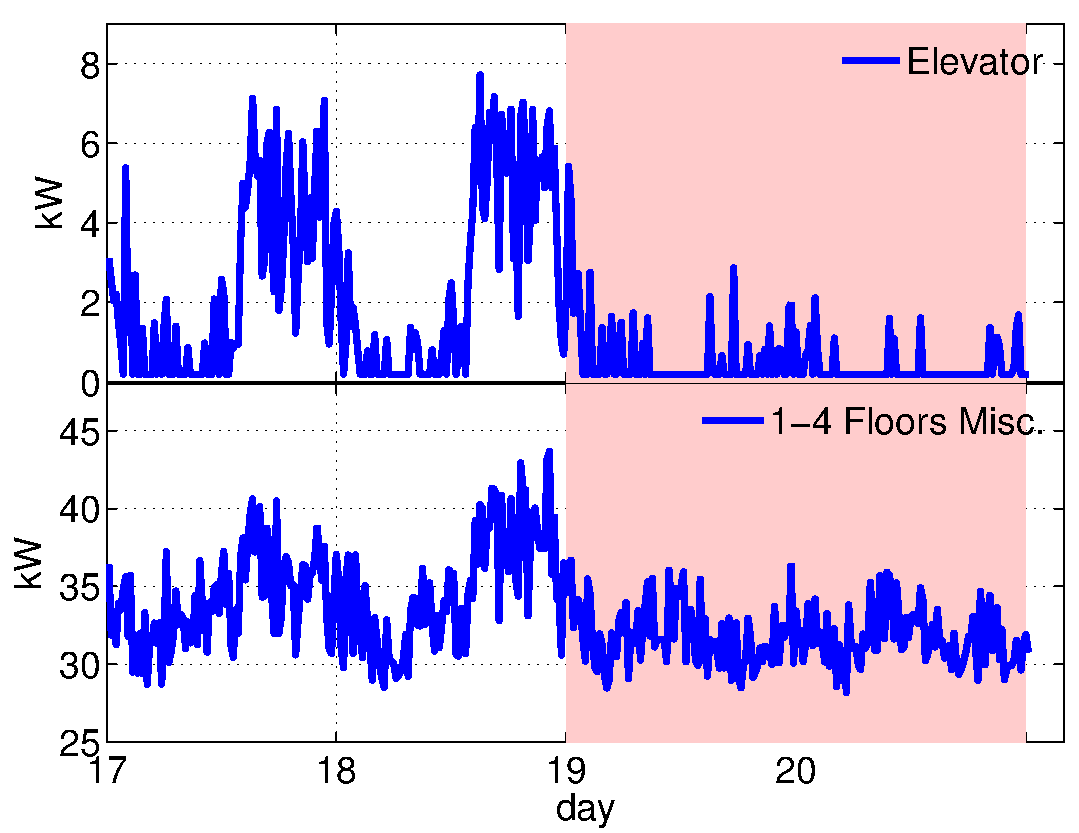
\includegraphics[width=.32\textwidth]{img/1sig7_sig49alarm19-eps-converted-to.pdf}}
 \hspace{.015\textwidth}
 \subfloat[Normal power and elevator usage\label{fig:res:cory22}]{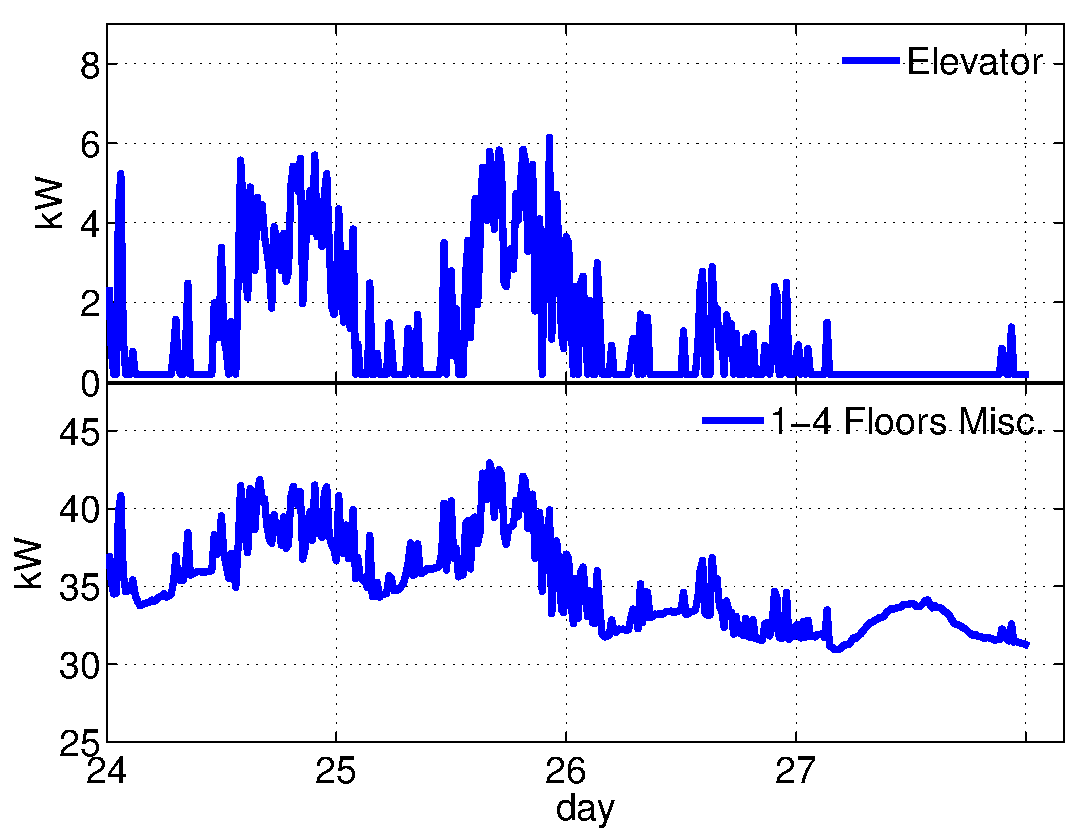
\includegraphics[width=.32\textwidth]{img/1sig7_sig49alarm-eps-converted-to.pdf}}\\ 
 \subfloat[Long term high power usage due to competing heating and cooling\label{fig:res:cory3}]{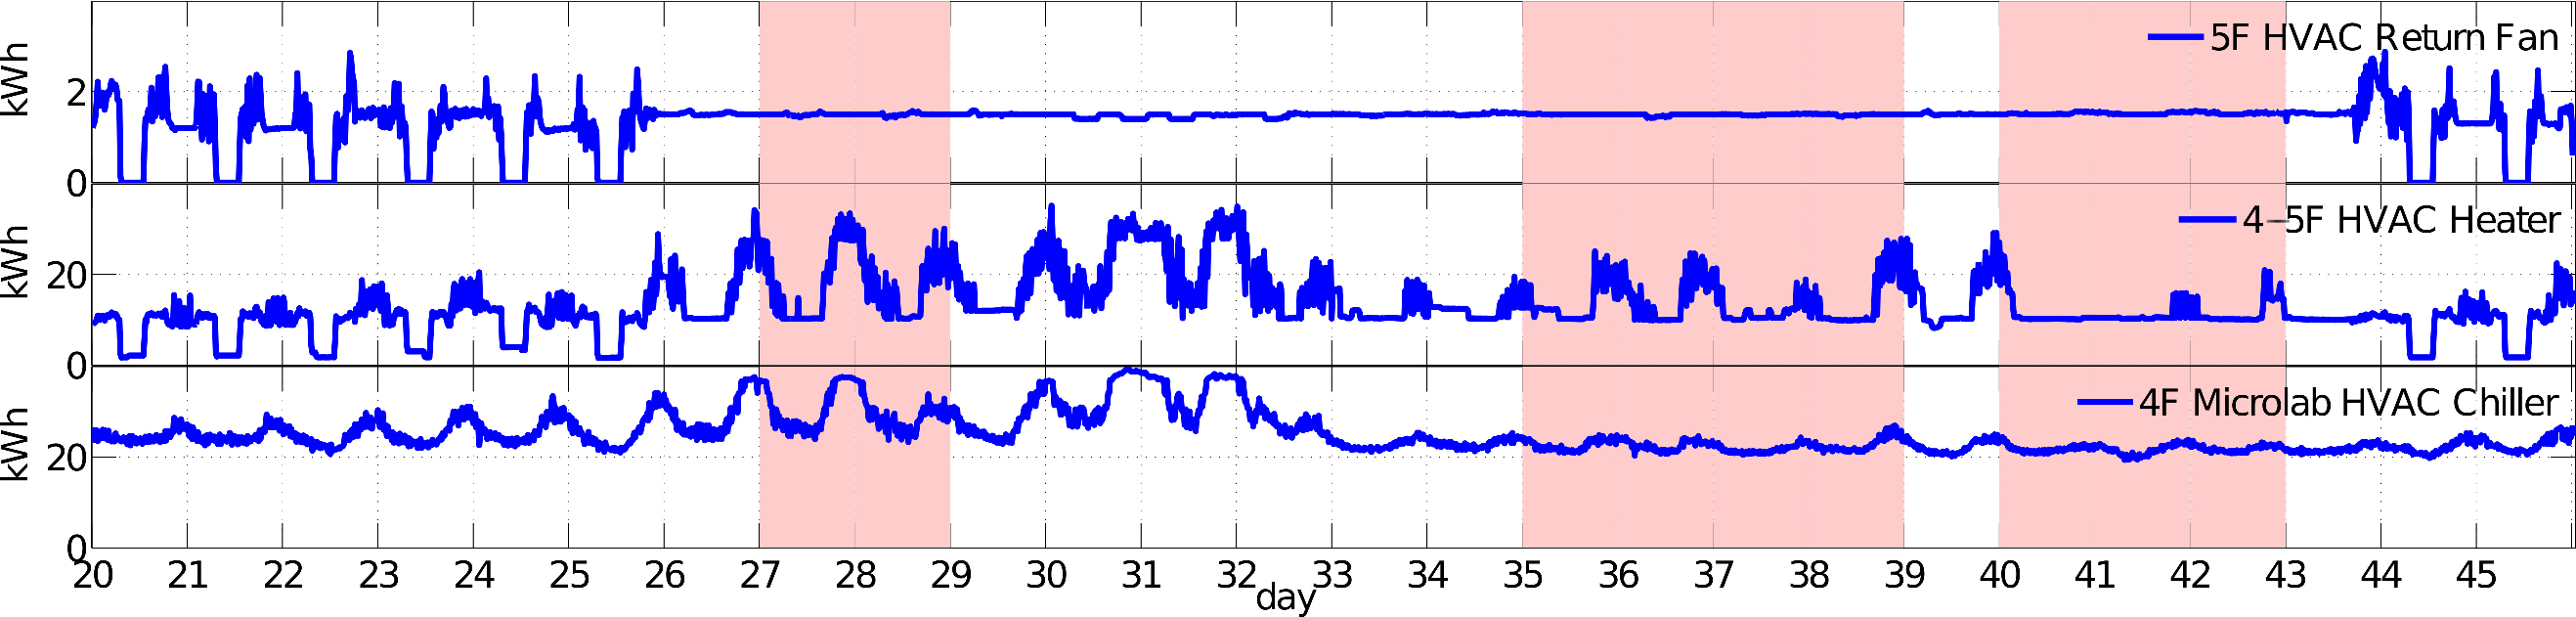
\includegraphics[width=\textwidth]{img/1sig34_sig54alarm27-eps-converted-to.pdf}} 
\caption{Example of alarms (red rectangles) reported by SBS on the Building 2 dataset}
\end{figure*}

In spite of the post-Fukushima measures to reduce Building 1 energy consumption, 
SBS reported 9 alarms corresponding to high power usage (Table \ref{tab:classif}).
Figure \ref{fig:res:eng1} depicts the electricity consumption of the light and EHP in the same room where two alarms are raised.
Because the EHP was not used during daytime (but is turned on at night, when the light is turned off) the relationship between the two devices 
is ``broken'' and an alarm is raised for each device.
Figure \ref{fig:res:eng2} shows another example of energy waste.  The light is on at night and the EHP is off.
The top-priority anomaly reported by SBS is caused by the 10 days long constant use of an EHP (Figure \ref{fig:res:eng4}) and this 
waste of electricity accounts for 165 kWh.
SBS partially reports this anomaly but lower values of $\tau$ permits us to identify most of it.


We observed 6 alarms corresponding to abnormally low power use.  Upon further inspection we notice that it corresponds to energy saving
 initiatives from the occupants -- likely due to electricity concerns in Japan.
This behavior is displayed in Figure \ref{fig:res:eng3}.  The room is occupied at the usual office hours (indicated by light usage)  but the 
EHP is not on in order to save electricity.

\subsubsection{Building 2}
SBS reported 39 alarms for the Building 2 dataset (Table \ref{tab:classif}).
 7 are classified as low power usage, however, our inspection revealed that the root causes are different than for the Building 1 dataset.
We observe that the low power usage usually corresponds to device failures or misconfiguration.  
For example, Figure \ref{fig:res:cory1} depicts the electricity consumption of the $2^{nd}$ floor chiller and a power riser that comprises the consumption of multiple systems, including the chiller.
As the chiller suddenly stops working, the correlation between both measurements is significantly altered and an alarm for each device is raised.

SBS also reports 25 alarms corresponding to high power usage. 
One of the identified anomalies is particularly interesting.
We indirectly observe abnormal usage of a device from the power consumption of the elevator and a power panel for equipment from 
the $1^{st}$ to the $4^{th}$ floor.
Figure~\ref{fig:res:cory21} and~\ref{fig:res:cory22} show the electricity consumption for both devices. 
SBS uncovers the correlation between the these two signals, as the amount of electricity going through the panel fluctuates along with the elevator power consumption (Figure \ref{fig:res:cory22}).
In fact, the elevator is a good indicator of the building's occupancy.
Anomalous energy-consumption is identified during a weekend as the consumption measured at the panel is independently fluctuating from the elevator usage.
These fluctuations are caused by a device that is not directly monitored.  Therefore, we could not identify the root cause more precisely. 
 Nevertheless, the alarm is worthwhile for building operators to start investigating.

The most important anomaly identified in Building 2 is shown in Figure \ref{fig:res:cory3}.
This anomaly corresponds to the malfunctioning of the HVAC heater serving the $4^{th}$ and $5^{th}$ floors. 
The heater is constantly working for 18 consecutive days, regardless of the underlying occupant activity.
Moreover, in order to maintain appropriate temperature this also results in an increase of the $4^{th}$ floor HVAC chiller power consumption 
and several fans, such as the one depicted in Figure \ref{fig:res:cory3}.
This situation is indicative of simultaneous heating and cooling -- whereby heating and cooling systems are competing -- and it 
is a well-know problem in building management that leads to significant energy waste.
For this example, the electricity waste is estimated around 2500 kWh for the heater.
Nevertheless, as the anomaly spans over 18 days, it is hidden in the building's overall consumption, thus, it is difficult to detect 
by building administrators without SBS.


\section{Related work}
Reducing the buildings energy consumption is an serious concern that received a lot of attention from the research community.
Since HVACs are one of the major consumer of electricity in the buildings, several researchers have mainly focused on reducing the consumption of HVACs.
The most promising techniques are based on occupancy model predictions to ensure that empty rooms are not over conditioned needlessly.
The room occupancy is usually monitored through sensor networks \cite{agarwal:ipsn2011,erickson:ipsn2011} or the computer network traffic \cite{kim:buildsys2010}.
These approaches are highly effective for buildings that have rooms rarely occupied (e.g. conference room).
For example, in Ref.~\cite{erickson:ipsn2011} the authors claim that such approach achieves 42\% annual energy saving.
However, these occupancy model predictions track human activity through sensor networks that imply the cost of an extra deployment and privacy concerns.
Fundamentally different, the approach proposed in this article prevents devices abnormal usages rather than optimizing the devices normal usage, nevertheless, the two approaches are complementary and can be used together.
% The main additional advantage of our approach is to analyze more than the HVAC activity without the need of extra sensors.

Energy wastes are also detected by predicting the future devices consumption using weather variables and regression analysis.
For example, using kernel regression one can forecasts the devices consumption and those that are significantly different from the predictions are reported as anomalous \cite{brown:buildperf2012}.
However, these approaches are particularly difficult to implement in real situations as they require training dataset and non-trivial parameter tuning.

Similar to our approach, several prior works take advantage of unsupervised anomaly detection methods to identify energy wastes.
These methods formalize the devices consumption, for example using the Fourier transform \cite{Bellala_buildsys11,wrinch:pes2012}, and detect outlier usually using simple statistics \cite{li:ieee2010} or clustering techniques \cite{bellala:kdd2012,jakkula,chen:aaaiw2011}.
However, these methods assume a certain periodicity in the data, thus, they report usages that appear at unusual times and may not correspond to a faulty operation.
In this article we do not make any assumption on the devices usage schedule but on the relationships between devices usage.

% Therefore, it is a practical way of reducing the energy consumption of any building in contrast to the anomaly detectors based on neural networks or kernel regression that requires training datasets and complex parameter tuning \cite{brown:buildperf2012}.
% Also, the proposed method does not require extra deployments such as sensors monitoring the room occupancy \cite{agarwal:ipsn2011,erickson:ipsn2011} or extra measurements for occupancy models (e.g. network traffic).
% 
% 
% This approach provides new insights in buildings energy consumption as it is fundamentally different from past works.
% complementary to other methods decreasing the energy consumption of the building normal operations.
% 
% it is more general (not only HVAC)
% 
% TODO look at IPSN TPC papers. Andreas Krause?

% 
% problem:
% The building energy consumption is mainly driven by its occupancy.
% The human occupancy is responsible for the majority of the devices energy consumption.
% For example, workstations, lights and air conditioners are utilized the most when humans occupied the building.
% 
% Thereby, all devices follow the same trend which is conducted by the human occupancy.
% In practice sensors data look all same.
% All devices are used during office hours and left off at night. (TODO see figure...)
% For our purpose, finding devices used simultaneously, this data is really difficult to analyze as the differences between each device is insignificant.
% 
% Our approach consists of; (1) subtract from the data the general trend driven by the building occupancy, (2) analyze remaining data to cluster devices used in concert.
% 
% 
% 
% result summary:
% We evaluate the proposed correlation estimator using 10 weeks of data from 135 devices serving 231 rooms.
% 
% contributions
% and advantages: unsupervised approach, small number of parameter (only one!), no training data required, no need of occupancy model/instrumentation, No distinction of weekdays, weekend, holidays...
% 

\section{Discussion}
The additional advantages of the work presented in this article are discussed in this section.

%practical
Since SBM mines in an unsupervised manner the devices relationships the proposed method is truly practical. 
In this work we validated the SBM efficiency using the sensors metadata (i.e. device types and location), however, these tags are not needed by SBM to uncover devices relationships.
Furthermore, SBM requires no prior information on the analyzed building and deploying our tool to other buildings requires no particular human intervention.
In particular the proposed approach do not need extra sensor deployment such as occupancy sensors. 

%best effort
Nevertheless, the proposed method takes advantage of all the existing building sensors.
The understanding of the building energy consumption is obviously better understand by sensing the consumption of numerous devices, 
but saving opportunities is observable with a minimum of 2 monitored devices.
This best effort approach is particularly effective as it requires no extra instrumentation that is also consuming electricity.
For example, our experiments revealed that the building occupancy is indirectly monitored by certain devices that betray the presence of humans (e.g. the elevator in the Cory Hall). 
Thereby, the proposed method would benefits from existing sensors that monitor the rooms occupancy (e.g. those deployed in \cite{agarwal:ipsn2011,erickson:ipsn2011}) albeit they are no needed.


%EMD
We also observed advantages of decomposing sensor data using EMD that is beneficial for different purpose.
In this article we analyze only the data at the medium frequencies, however, we observed that data at the high frequencies and residual data (Figure \ref{fig:heatmap}) permit to discriminate the type of the monitored devices.
Consequently, this information is valuable to automatically retrieve the semantic of the devices.


% %limitation
% The goal of this article is to develop an unsupervised tool that identifies energy wastes in buildings.
% However, the design of the system that reports these energy waste in real time is beyond the goal of this work.
% more work is needed to allow on line detection: use of smaller time bin.
% 
% 
% season changes; devices relationships have seasonal pattern thus we may need forecast models such as ARIMA to make the reference matrix evolve in time.




\section{Conclusion}
The goal of this article is to provide to building administrators tools that assist them to prevent electricity waste.
Consequently, we proposed a new approach to systematically detect abnormal energy-consumption in buildings, the Strip, Bind, and Search (SBS) method.
SBS uncovers the inter-device usage patterns by striping dominant trends off the traces.
Then, it monitors the devices usage and report misbehaving devices.
Our main contribution is to develop an unsupervised technique to uncover the devices intrinsic relationships that are hidden by the noise and dominant patterns inherent to the sensor raw data.
This technique makes the proposed tool really practical as demonstrated by our evaluation using data from two buildings that have fundamentally different infrastructures.
Different types of energy waste are identified in this two buildings. 
The most important one being an instance of competing heater and cooler that caused the heater to waste around 2500~kWh.



% \section*{Acknowledgment}
% The authors thank Hideya Ochiai for providing the data from the Green University of Tokyo Project.


\small
\bibliographystyle{abbrv}
\bibliography{references}
\end{document}